\documentclass[12pt]{jarticle}

\usepackage[dvipdfmx]{graphicx}
\usepackage{url}
\usepackage{listings,jlisting}
\usepackage{ascmac}
\usepackage{amsmath,amssymb}
\usepackage{comment}

%ここからソースコードの表示に関する設定
\lstset{
  basicstyle={\ttfamily},
  identifierstyle={\small},
  commentstyle={\smallitshape},
  keywordstyle={\small\bfseries},
  ndkeywordstyle={\small},
  stringstyle={\small\ttfamily},
  frame={tb},
  breaklines=true,
  columns=[l]{fullflexible},
  numbers=left,
  xrightmargin=0zw,
  xleftmargin=3zw,
  numberstyle={\scriptsize},
  stepnumber=1,
  numbersep=1zw,
  lineskip=-0.5ex
}
%ここまでソースコードの表示に関する設定

\title{知能プログラミング演習II 課題2}
\author{グループ8\\
	29114003 青山周平\\
	29114060 後藤拓也\\
	29114116 増田大輝\\
	29114142 湯浅範子\\
	29119016 小中祐希\\
%{\small (グループレポートの場合は、グループ名および全員の学生番号と氏名が必要)}
}
\date{2019年10月25日}

\begin{document}
\maketitle

\paragraph{提出物} rep2,group08.zip
\begin{comment}
\paragraph{グループ} グループ8
\paragraph{メンバー}
\begin{tabular}{|c|c|}
  \hline
  学生番号&氏名\\
  \hline\hline
  29114003&青山周平\\
  \hline
  29114060&後藤拓也\\
  \hline
  29114116&増田大輝\\
  \hline
  29114142&湯浅範子\\
  \hline
  29119016&小中祐希\\
  \hline
\end{tabular}
\end{comment}

\section{課題の説明}
\begin{description}
\item[課題2-1] MatchingクラスまたはUnifyクラスを用い,パターンで検索可能な簡単なデータベースを作成せよ.
\item[課題2-2] 自分たちの興味ある分野の知識についてデータセットを作り,上記2-1で実装したデータベースに登録せよ.また,検索実行例を示せ.どのような方法でデータセットを登録しても構わない.
\item[課題2-3] 上記システムのGUIを作成せよ. \\
・データの追加,検索,削除をGUIで操作できるようにすること. \\
・登録されたデータが次回起動時に消えないよう,登録されたデータをファイルへ書き込んだり読み込んだりできるようにすること.
\end{description}

\section{必須課題2-1}
\begin{screen}
  MatchingクラスまたはUnifyクラスを用い,パターンで検索可能な簡単なデータベースを作成せよ.
\end{screen}
私の担当箇所は,データセットからデータを読み取り,データベースに格納するためのメソッドの作成である.

\subsection{手法}
課題内容の実装のために,以下のように改良を加えた.

\begin{enumerate}
\item 与えられたデータセットをDBに格納する.
\item DBにアクセスするためのDAOを作成する.
\item DBから得られたデータと,検索文を比較して検索を行えるようMatching.javaとUnify.javaを改良する.
\end{enumerate}

1.に関して,テキストファイルとDB間でデータのやり取りを行うため,テキストファイルにアクセスするためのjavaファイルTextCon.javaを作成した.そして1.の実現のため,テキストファイルからデータを読み込むためのメソッドreadTextFileを作成した.これは私が担当した.

2.に関しては,DBアクセスを行う際のデザインパターンであるDAOの作成のため,TextDAO.javaを作成した.具体的にはtable(texts)を作成し,columnとしてuuid(int型)とline(text型)を定め,そこにテキストファイルの中身が入るようにした.これも私が担当した.

3.に関しては,与えられたUnify.javaでは変数入力の際に値を返すことが出来ないため,変数検索にも対応可能になるようプログラムの書き換えを行った.これは後藤君と小中君が担当した.

\subsection{実装}
まずテキストファイルからDBを利用するためのプログラムを作成した.始めにDBとそのtableを作成し,その内容を初期化する.その後与えられた「テキストファイルに対する操作のプログラム」を利用してテキストファイルから一文ずつ取り出しDBに格納する.\par
このとき,テキストファイルを読み込むためのメソッドはreadTextFile,DBとそのtableを作成するメソッドがcreateTab,DBのtable内部を初期化するメソッドがdeleteData,読み込んだデータをDBに格納するメソッドがinsertTextTabである.\par
テキストファイルアクセスとDBアクセスを分けるため,それぞれTextCon.java,TextDAO.javaというファイルを作成し,readTextFileメソッドはTextCon.javaに,createTab,deleteData,insertTextTabメソッドはTextDAO.javaに含まれている.\\

また,DBアクセスプログラムは,3年生前期の授業で取ったプログラミング応用の課題で作成したDAOなどのプログラムも参考にして作成を行った.\\

テキストファイルを読み込んでDBアクセスを指示するreadTextFileメソッドの実装をソースコード\ref{readTextFile}に示す.
\begin{lstlisting}[caption=readTextFileメソッド,label=readTextFile]
public void readTextFile() throws FileNotFoundException{
	String empty = "";
	//textファイル処理
	try {
		// tableの作成【DB】
		TextDAO.createTab();
		TextDAO.conCom();
		// tableの中身の初期化【DB】
		TextDAO.deleteData();

		// ファイル読み込み操作
			・・・
			if (!line.equals(empty)) {
				// 更新【DB】
				TextDAO.insertTextTab(line);
			}
			//【DB】
			TextDAO.conCom();
		}
		in.close();  // ファイルを閉じる
	} catch (IOException e) {
		e.printStackTrace();
	}
	//【DB】
	TextDAO.conCom();
	TextDAO.closeConn();
}
\end{lstlisting}

DBのtable作成のためのcreateTabメソッドをソースコード\ref{createTab}に示す.
\begin{lstlisting}[caption=createTabメソッド,label=createTab]
public static Connection conn = null;
public static final String connDB = "jdbc:sqlite:data.db";
// 格納用tableを作成
public static void createTab(){
	PreparedStatement pStmt = null;
	String sql;
	try{
		Class.forName("org.sqlite.JDBC");
		conn = DriverManager.getConnection(connDB);
		conn.setAutoCommit(false);
		sql = "create table texts(uuid int, line text)";
		pStmt = conn.prepareStatement(sql);
		pStmt.executeUpdate();
	}catch{
		・・・
	}
}
\end{lstlisting}

DBのtableの中身の初期化のためのdeleteDataメソッドをソースコード\ref{deleteData}に示す.
\begin{lstlisting}[caption=deleteDataメソッド,label=deleteData]
// DBtableの中身の削除
public static void deleteData() {
	conn = null;
	PreparedStatement pStmt = null;
	try{
	    Class.forName("org.sqlite.JDBC");
	    if(conn == null){
			 conn = DriverManager.getConnection(connDB);
			 conn.setAutoCommit(false);
		}
    	String sql = "delete from texts";
    	pStmt = conn.prepareStatement(sql);
   		pStmt.executeUpdate();
	}catch{
		・・・
	}
}
\end{lstlisting}

DBにデータを格納するためのinsertTextTabメソッドをソースコード\ref{insertTextTab}に示す.
\begin{lstlisting}[caption=insertTextTabメソッド,label=insertTextTab]
// tableに追加
public static void insertTextTab(String line) {
	PreparedStatement pStmt = null;
	String sql;
	try{
		Class.forName("org.sqlite.JDBC");
		if(conn == null){
			 openConn();
		}
		sql = "insert into texts values(?, ?)";
		pStmt = conn.prepareStatement(sql);
		pStmt.setInt(1, id);
		pStmt.setString(2, line);
		pStmt.executeUpdate();
		id++;
	}catch{
		・・・
	}
}
\end{lstlisting}

またこれらの動作のため,DBへのコネクションOPENとしてopenConnメソッド,CLOSEとしてcloseConnメソッド,COMMITとしてconComメソッドを新たに作成している.これらはTextDAO.javaとTextCon.javaのどちらからも利用される.

\subsection{実行例}
作成したDBへの格納プログラムが正しく動作しているかを確認するためにTest.javaを作成し,readTextFileメソッドを実行した.すると,data.dbという名前のDBが作成される.この中身を確認したところ,以下のように表示された.
\begin{lstlisting}
C:\Users\Owner>sqlite3 data.db
SQLite version 3.28.0 2019-04-16 19:49:53
Enter ".help" for usage hints.
sqlite> .table
texts
sqlite> select * from texts;
1|Hanako is a girl
2|Hanako is a student
3|student is a kind of human
4|human is a kind of mammal
5|Hanako has a hobby of playing video-games
6|Hanako has a hobby of playing air-guitar
7|Hanako studies philosophy
8|Hanako loves Taro
9|Taro is a boy
10|Taro is a student
11|Taro has a hobby of playing video-games
12|Taro studies informatics
13|Taro loves Jiro
14|Taro has a pet named Jiro
15|Jiro is a boy
16|Jiro is a dog
17|dog is a kind of mammal
18|Jiro has a hobby of playing frisbee
19|Jiro loves Hanako
sqlite>
\end{lstlisting}
この結果はテキストファイルに含まれていたデータセットの内容と一致することから,作成したプログラムが正しく動作し,DBが作成できていることが確認できた.

\subsection{考察}
この課題は課題文の解釈の方法がいくつか考えられたため,どのようにDBを作成するかを考えるのにかなりの時間を要した.\\

まず,DBの作成を行うため,データセットであるテキストファイルからどのようにDBを作成するかを考えた.この時大きく分けて2種類の作成方法がまず考えられた.それを以下に示す.
\begin{enumerate}
\item DBにデータセットと同様の内容を格納する.
\item DBにUnifyで処理した検索文(変数を含む文章)とその出力結果を格納する.
\end{enumerate}
この2種類の考えは,課題文の解釈の違いによって考えられた.\par
「MatchingクラスまたはUnifyクラスを用い,パターンで検索可能な簡単なデータベースを作成せよ.」という課題であるが,MatchingクラスやUnifyクラスをどの段階で使用するのかが明確に判断できず,DB作成後にMatchingクラスやUnifyクラスを利用するのか,MatchingクラスやUnifyクラスを利用して得られた結果をDBに格納するのかが分からなかったからである.MatchingクラスやUnifyクラスを使用する前にDBを作成する場合は1.\ のDBの形式にし,MatchingクラスやUnifyクラスを使用した後にDBを作成する場合は2.\ のDBの形式にすると考えられたが,どちらを採用するかがかなり難しい判断であった.\\

さらに,DBをデータセットと同様の内容とした場合はさらに3種類の作成方法が考えられた.それを以下に示す.
\begin{enumerate}
\item DBに一文をそのままtext型として格納する.
\item DBに一文を各単語毎に分割して格納する.
\item DBで動詞毎にtableを作成し,それぞれの動詞で分類分けした状態で主語とそれ以外(動詞も除く)に分割して格納する.
\end{enumerate}
DBをより効率よく利用する方法を考え,これらのような格納方法を考えた.\\

DBの作成方法に複数の方法が考えられたが,これは必須課題の1つ目であり,作成期間も一週間と短く,出来るだけ早く方針を固めなければならない.そこで私たちの班では,DBのこれ以降の課題との関係性や検索方法と課題文の内容にどれだけ沿うことが出来るかなどを考慮してプログラムを作成することとした.\\

ここで,先に挙げたDBの格納方法とその具体例を表形式にまとめ,それぞれの利点と欠点を上げていく.\par
1つ目は「DBに一文をそのままtext型として格納する.」方法である.\\

\begin{table}[htb]
  \begin{center}
    \caption{DB例1(table:texts)}
    \begin{tabular}{|c|c|} \hline
      uuid(int) & line(text) \\ \hline \hline
      1 & Hanako is a girl \\ \hline
      2 & Hanako is a student \\ \hline
      ・・・ & ・・・ \\ \hline
	  8 & Hanako loves Taro \\ \hline
    \end{tabular}
    \label{tab:ex1}
  \end{center}
\end{table}

表\ref{tab:ex1} の利点は,DBへの格納が単純であるため比較的楽にプログラムすることが出来る点にある.また,Unify.java等がデータを受け取るときにテキストファイルを読み込む形と殆ど変わらずにプログラム出来るため,改良の手間が少し減る点もあげられる.\par
これに対し欠点は,格納方法がテキストファイルと同様の形式であるため,DBへ格納した恩恵をあまり得られない点にある.データの削除や追加はテキストファイルよりも楽に行うことが出来るが,検索に関しての手間はテキストファイルと変わらないため,あまり意味のないDBになってしまう可能性も考えられる.\\

%\vspace{5mm}
2つ目は「DBに一文を各単語毎に分割して格納する.」方法である.\\


\begin{table}[htb]
  \begin{center}
    \caption{DB例2(table:texts)}
    \begin{tabular}{|c|c|c|c|c|} \hline
      uuid(int) & namea(text) & nameb(text) & namec(text) & named(text) \\ \hline \hline
      1 & Hanako & is & a & girl \\ \hline
      2 & Hanako & is & a & student \\ \hline
      ・・・ & ・・・ & ・・・ & ・・・ & ・・・ \\ \hline
	  8 & Hanako & loves & Taro & NULL \\ \hline
    \end{tabular}
    \label{tab:ex2}
  \end{center}
\end{table}

表\ref{tab:ex2} の利点は,検索がDBを用いて行うことが出来るために,マッチング操作にかかる手間が大幅に減ることがあげられる.\par
これに対し欠点は,一文に含まれている単語の数が一定でないため,上の表のようにフィールドによってはNULLになってしまいDBへの格納が複雑になることがあげられる.一文が分割される単語数もテキストファイルに含まれる行数も可変であるため,可変長二次元配列を活用して格納を行わなければならなくなってしまい,かなり複雑なプログラムとなることが考えられる.またこの格納方法では,検索時にDB参照によって検索結果を得られるため,使用するように指定されているMatchingクラスやUnifyクラスが利用できなくなってしまうことも欠点としてあげられる.\\

3つ目は「DBで動詞毎にtableを作成し,それぞれの動詞で分類分けした状態で主語とそれ以外(動詞も除く)に分割して格納する.」方法である.\\

\begin{table}[htb]
  \begin{center}
    \caption{DB例3(table:iss)}
		\begin{tabular}{|c|c|c|} \hline
	   uuid(int) & namea(text) & nameb(text) \\ \hline \hline
		  1 & Hanako & a girl \\ \hline
		  2 & Hanako & a student \\ \hline
		  ・・・ & ・・・ & ・・・ \\ \hline
	 \end{tabular}
    \label{tab:ex3}
  \end{center}
\end{table}


\begin{table}[htb]
  \begin{center}
    \caption{DB例3(table:lovess)}
	\begin{tabular}{|c|c|c|} \hline
	 uuid(int) & namea(text) & nameb(text) \\ \hline \hline
	8 & Hanako & Taro \\ \hline
	・・・ & ・・・ & ・・・ \\ \hline
	\end{tabular}
    \label{tab:ex4}
  \end{center}
\end{table}

表\ref{tab:ex3}, 表\ref{tab:ex4} の利点は,tableを複数作成することで,テキストファイルには出来ない単語毎の分類が可能になるので,DBを利用する利点が明確になることである.同時に,分類分けが行われることで検索時のマッチング操作にかかる手間が減ることも考えられる.\par
これに対し欠点は,分割を行って動詞毎にtableを作成するため,DAOが非常に複雑になってしまうことがあげられる.実際にこのプログラムは始めに作成したが,デバッグ作業にかなりの時間を要することになった.また各table毎に検索を行うため,Unify.javaに引数としてデータを与える際に工夫が必要になることも,実行効率は良いが実装効率が悪いことを示している.さらに調べたところ,tableとして指定できない特定の文字列が存在し,それがisが該当していると分かった.そのため動詞毎でtableを作成する場合は全ての動詞に's'を付けるなどの工夫が必要になることが課題を解く中で分かった.これも,プログラムが複雑になる原因の一つとして考えられる.\\

最後に,「DBにUnifyで処理した検索文(変数を含む文章)とその出力結果を格納する.」方法である.\\

\clearpage

\begin{table}[htb]
  \begin{center}
    \caption{DB例4(table:answers)}
    \begin{tabular}{|c|c|c|} \hline
      uuid(int) & question(text) & answer(text) \\ \hline \hline
      1 & ?x has a hobby of playing video-games & Hanako, Taro \\ \hline
      2 & Hanako is a ?y & girl \\ \hline
      ・・・ & ・・・ & ・・・ \\ \hline
	  8 & ?x is a boy, ?x loves ?y & (Taro, Jiro), (Jiro, Hanako) \\ \hline
    \end{tabular}
    \label{tab:ex5}
  \end{center}
\end{table}

表\ref{tab:ex5} の利点は,必須課題で求めらているプログラムに最も近いと考えられるプログラムであることがあげられる.また,データセットとDBの役割の違いがはっきりするため,テキストファイルとDBを有効に活用できている部分も利点と考えられる.\par
これに対し欠点は,格納のためのプログラムが複雑になってしまうことと,発展課題を行う際に追加と削除のデータがDBに反映させられないことがあげられる.DBを利用することで,テキストファイルよりも追加や削除が簡単になるが,この方法で実装を行うとこれが出来ない.それにより追加や削除命令に応じてテキストファイルを直接操作することになるが,これは非常に手間がかかり効率も悪い.\\

これらの利点と欠点,そして実装期間を考え,私たちの班は表\ref{tab:ex1}の方法を採用することとした.これらを踏まえ作成したものが先に述べたプログラムである.そのため,結果としてDBはテキストファイルと形式を殆ど変えることなく作成することとなった.ただしこのとき,改行はDBに含まないことにしたため,DBでは空行は含まれずに格納される.\par
これにより実装を分担して行う今回のような課題は実装方法が複雑にならなかったことから大幅に時間をかけることなくプログラムを作成することが出来た.\\



\section{課題2-1(-1)}
\begin{screen}
与えられたパターンにマッチする全データを列挙するプログラムを作成せよ.\\
例えば,この例のような形式のデータセットから,?x has a hobby of playing video-games や Hanako is a ?y のような,様々なパターンにマッチするデータを検索できるようにすること.
\end{screen}

\subsection{手法}
Matching.javaでのマッチングの大まかな手順は次のようになる.\\
また,今回はサンプルプログラムとして用意されているMatching.javaを必要に応じて書き換えることによりマッチングを実現した.

\begin{enumerate}
\item Matchingクラスを定義し,Matcherクラスのインスタンスを生成する
\item 引数にとった二つの文章が等しいかどうか比較する
\item 文章をトークンごとに分割し,トークンの数を比較する
\item トークンごとの比較をする
\item トークンの片側に変数が含まれていたらハッシュに登録されているかを確認し,未登録であれば格納する
\item 他のトークンが全てマッチング成功したら,変数に対応するトークンを出力する
\end{enumerate}


\subsection{実装}
今回用意されていたMatching.javaにはマッチングに必要なメソッド自体はすでに含まれていたが,返り値が全てbooleanであったため,マッチングの結果を出力できるように書き換えた.\\

まず,プレゼンターとのやり取りを行うためにmainメソッド内に必要な要素を追加した.\\
また,テキストの読み込み等はプレゼンター側で行うため削除し,テスト実行用として出力文を追加している.(ソースコード1)
\begin{lstlisting}[caption=mainメソッドの変更, label=mid]
List<String> answer = new ArrayList<String>(); // 答えを格納

	View view = new View(); // インスタンス?の作成
	Presenter presenter = new Presenter(view);

	presenter.start(); // DBの作成

	presenter.searchData(arg[0]); // 検索語入力
	answer = view.getSr(); // 答えを取得

	//answer.add((new Matcher()).matching(arg[0],line));//ここでarg[0]引数1, arg[1]に引数2

	//テスト出力用
	for(int i = 0; i < answer.size(); i++) {
		if(answer.get(i) != " ") {
			System.out.println("★answer = " + answer.get(i));
		}

	}
\end{lstlisting}

次に,マッチングした結果を実際に出力できるようにするための変更点を示す.\\
MatcherクラスやMatcherクラスのインスタンスを定義する部分では,新しく変数flagやリストKeyListを追加している.(ソースコード2)
\begin{lstlisting}[caption=追加要素, label=mid]
class Matcher {
	  StringTokenizer st1;
	  StringTokenizer st2;
	  HashMap<String,String> vars;
	  ArrayList<String> KeyList;  //Keyをとり,HashMapのValueを取るためのリスト
	  int flag;	//ミスフラグ

	  Matcher(){
		vars = new HashMap<String,String>();
		KeyList = new ArrayList<String>();
		flag = 0;
	  }
\end{lstlisting}

matchingメソッドでは,booleanではなくマッチング結果(String)を返したいので,メソッドをString型に変更した.\\
マッチングが成功した場合は該当のトークンを,出力がない(完全一致,マッチングに失敗など)場合は空白を返している.(ソースコード3)
\begin{lstlisting}[caption=matchingメソッド, label=mid]
public String matching(String string1,String string2){
		//System.out.println("tagetData = " + string1);
		//System.out.println("resultList = " + string2);

		// 同じなら成功
		if(string1.equals(string2)) return " ";

		// 各々トークンに分ける
		st1 = new StringTokenizer(string1);
		st2 = new StringTokenizer(string2);

		//System.out.println("トークンの数" + st2.countTokens());

		// 数が異なったら失敗
		if(st1.countTokens() != st2.countTokens()) return " ";

		// 定数同士
		for(int i = 0 ; i < st1.countTokens();){
		    if(!tokenMatching(st1.nextToken(),st2.nextToken())){
			// トークンが一つでもマッチングに失敗したら失敗
			return " ";
		    }
		}


		// 最後まで O.K. なら成功
		//System.out.println("成功!" + vars.get(KeyList.get(0)));
		return vars.get(KeyList.get(0));
	  }
\end{lstlisting}

varMatchingメソッドでは,初めてトークンがvarに追加される際にリストKeyListにvartokenを追加することでマッチングの答えを取得,保持している.(ソースコード4)
\begin{lstlisting}[caption=varMatchingメソッド, label=mid]
public boolean varMatching(String vartoken,String token){
		if(vars.containsKey(vartoken)){
		    if(token.equals(vars.get(vartoken))){
		    	//System.out.println(token);
			return true;
		    }
		    else {
			return false;
		    }
		} else {
		    vars.put(vartoken,token);
		    KeyList.add(vartoken);
		    //System.out.println(vars.get(vartoken));
		}
		return true;
	  }
\end{lstlisting}

\subsection{実行例}
今回は以下のデータセットを対象に,マッチングのみを行った例を示す.
\begin{lstlisting}[caption=データセット]
Hanako is a girl
Hanako is a student
student is a kind of human
human is a kind of mammal
Hanako has a hobby of playing video-games
Hanako has a hobby of playing air-guitar
Hanako studies philosophy
Hanako loves Taro
Taro is a boy
Taro is a student
Taro has a hobby of playing video-games
Taro studies informatics
Taro loves Jiro
Taro has a pet named Jiro
Jiro is a boy
Jiro is a dog
dog is a kind of mammal
Jiro has a hobby of playing frisbee
Shuhei is a boy
\end{lstlisting}

引数には以下の質問文を与えた.\\
"?x is a boy"\\

実行結果は以下のようになった.
\begin{lstlisting}[caption=実行結果]
Successfully started
targetData1 = ?x is a boy
検索結果を取得
★answer = Taro
★answer = Jiro
★answer = Shuhei
\end{lstlisting}


\subsection{考察}
今回の課題ではサンプルプログラムMatching.javaがあらかじめ用意されていたので,ここではサンプルプログラムをハンドトレースしていって理解するまでのプロセスにおいて感じたこと,考えたことを記す.\\
まずプログラムを見る前にイメージした手法だが,本課題において求められているパターン照合は単語単位でのマッチングが必要になってくるので,単にString型の文章同士を比較するのでは駄目だということが直感的にわかる.\\
ウェブインテリジェンスを履修していたので形態素解析が思いついたが,今回は英文なので単語間に空白があり,実際はそのことを利用してStringTokenizerで分割をしている.日本語などにも対応させようとすると形態素解析などの作業が必要になってくるのではないだろうか.\\
次にmatchingだが、トークンごとに比較する時に単に一致したら成功というだけでなく,片側が変数で片側が定数という場合を例外として扱わなければならない.今回のプログラムでは複数のboolean型のメソッドをうまく用いて課題通りのマッチングを実現しているが,返り値がbooleanなために実際に求めた単語を素直に返す,ということができなかった.ここが今回の2-1において一番やっかいな部分であったと感じた.\\
今回はメソッドの外に共通のリストを用意し,varMatchingの段階で格納,保持することで実現することができた.




\section{課題2-1(-2)}
\begin{screen}
複数のパターンが与えられたときに全ての可能な変数束縛の集合を返すようなプログラムを作成せよ.
例えば,上記の例で「?x is a boy」と「?x loves ?y」の両方が与えられたときに,(?x, ?y) の全ての可能な変数束縛の集合として{(Taro, Jiro), (Jiro, Hanako)}を返すこと.
\end{screen}

\subsection{手法}
課題を達成する(つまり, 「?x is a boy」と「?x loves ?y」と引数を取ると, {(Taro, Jiro), (Jiro, Hanako)}を返す)ために以下のようなプログラムの処理を行う.

\begin{enumerate}
\item 全体をまとめるハッシュマップを1つ生成する.
\item 1つ目の引数, 2つ目の引数を順番に処理を行う.
\item textファイルからデータセットを1行ずつ読み取り, 1行ずつ引数と照合する.
\item 1行はトークン単位に分割され, マッチングは各トークンごとで行う.
\item 対応した場合, ハッシュマップにKeyとして変数(?xや?yなど)を, Valueとして具体定数(TaroやJiroなど)を加えていく.
\item 1つ目の引数で束縛された変数は, 2つ目の引数に反映される(1つ目で?x=Taroと決まれば, 2つ目の引数ではその条件を引き継がせる).
\item ハッシュマップを2次元リストにし, 中身(Keyや各Keyに対応するVlaue)をリスト化することで, 全てのマッチング可能なパターンを1つのハッシュマップに格納できる.
\end{enumerate}

\begin{figure}[htbp]
 \begin{center}
  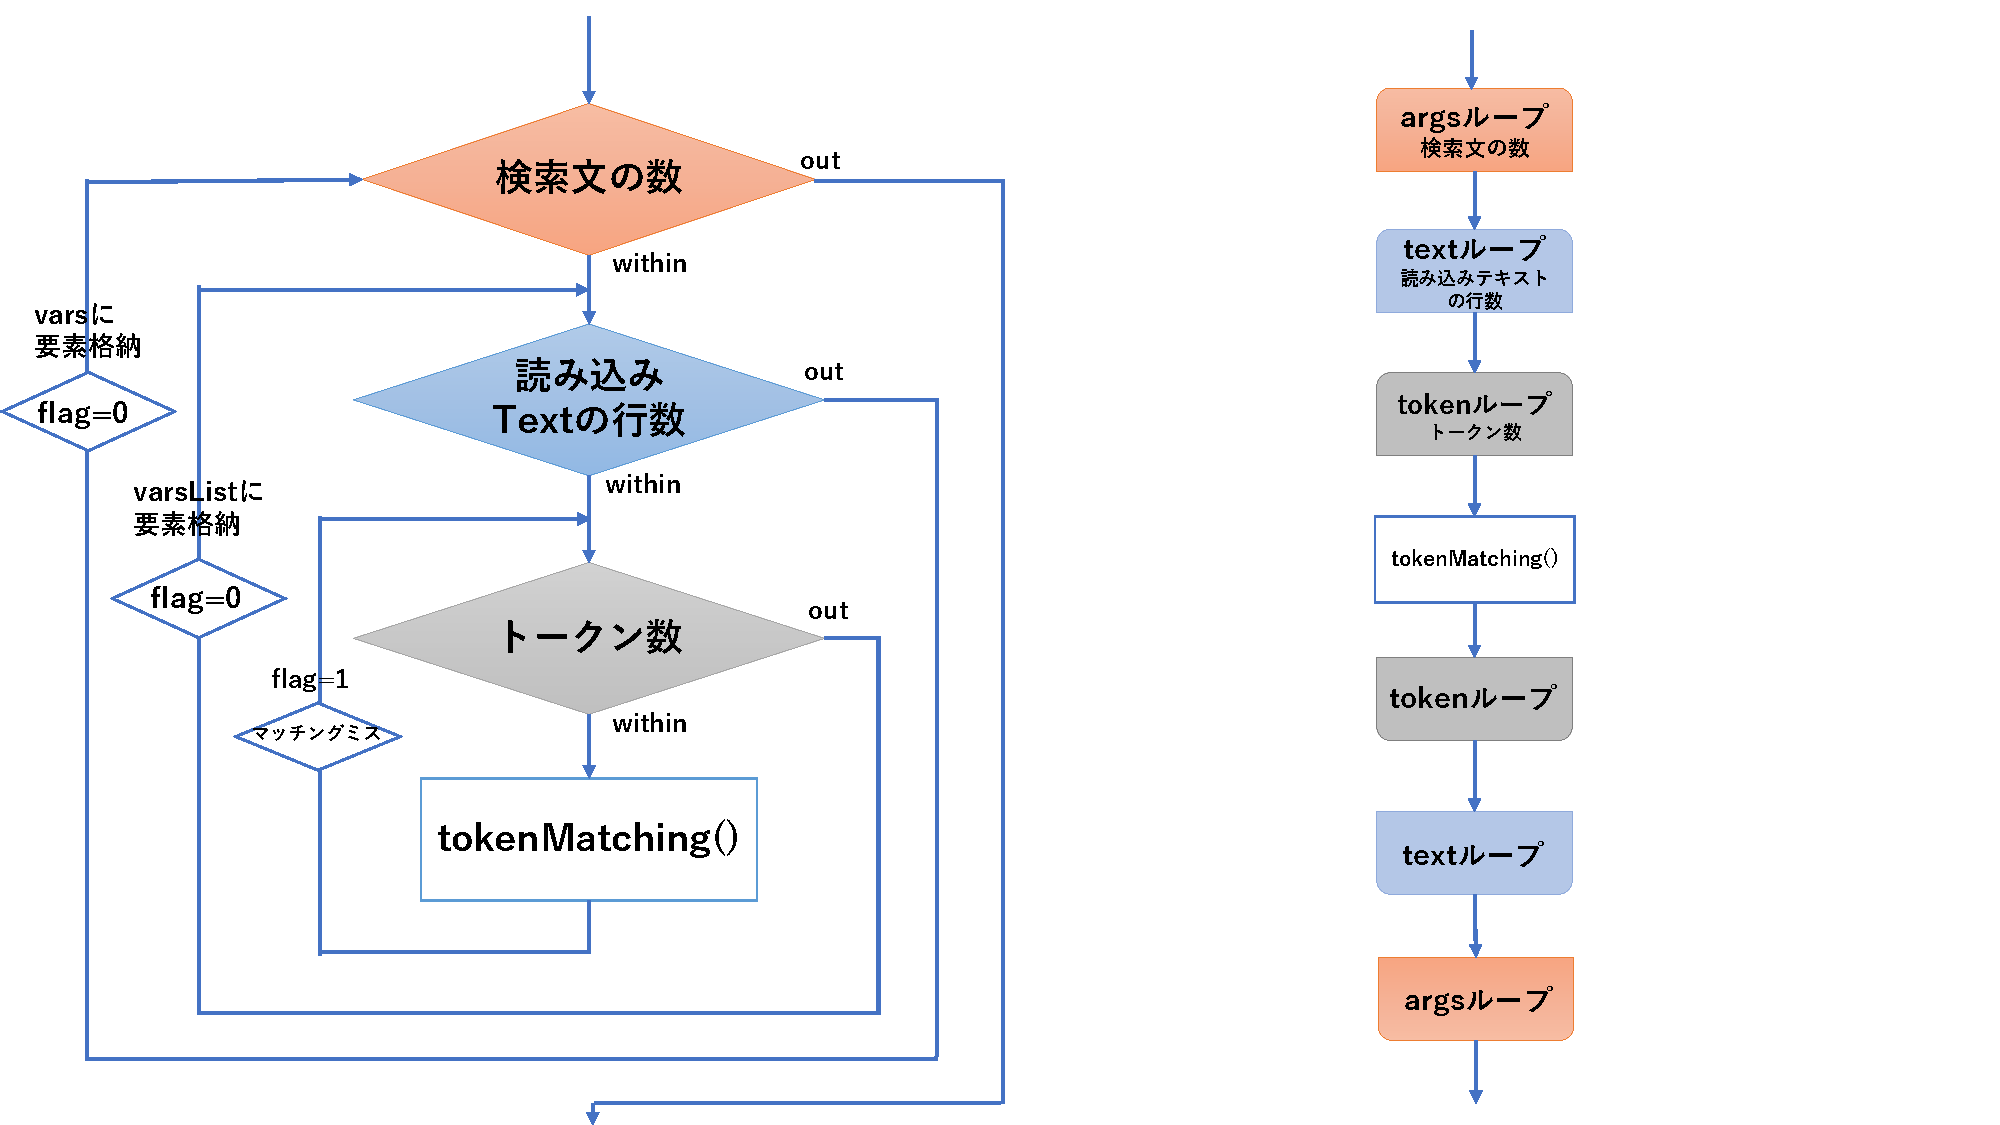
\includegraphics[width = 10cm, pagebox = cropbox, clip]{unify.pdf}
 \end{center}
 \caption[]{unifyプログラムの3つのループ}\label{fig:fig1.1}
\end{figure}

プログラムの流れは多段階のループ構造を構築している. 図1における"3つの大きなループ"を参照し, 上記の7つの手法について詳しく説明する.

1.に関して, mainクラスで1度Unifierクラスのインスタンスが生成されるとコンストラクタにより, ハッシュマップをはじめとするあらかじめ宣言されていた複数の変数やリストを初期化する. ここで初期化され生成されたインスタンスは, 今後のプログラム全体で使われる.

2.に関しては, 2つの引数をリストに格納させ, ループ処理を行う. ここが1つ目の大きなループである.

3.に関しては, BufferedReaderオブジェクトによりテキストを1行ずつ読み込む. ここが2つ目の大きなループである.

4.に関しては, 既存のプログラムを利用し, StringTokenizerにより分解したトークンの数だけループ処理をする. ここが3つ目の大きなループである. 引数と読みこんだ1行とでトークン数の異なる場合は, トークン数の多いほうにそろえるように, 少ないほうにnullを入れて数を調整する.

5.に関しては, トークン単位のマッチングは成功しても, 1行を通して成功していなければ成功とはいえない. 例えば, 「?x is a boy」と「Hanako is girl」は, トークン単位のループ処理ででマッチングをしていくと, 先に「?x = Hanako」でマッチングが成功するが, その後「boy != girl」となるので, 今回は失敗であり, ハッシュマップには追加できない. これを実現するために, 1行すべてのマッチングが成功した後に, これまで成功していたトークンの組をハッシュマップに保存する処理を行う. 具体的には, マッチングが成功したトークンの組はそれぞれ一時バッファならぬ一時リストに追加して, ハッシュマップには追加しない. マッチングの成功不成功を判断する"ミスフラグ"を用意し, 1行におけるトークンの組み合わせすべてが成功したら(ミスフラグが上がらなかったら), 先ほどの一時リストの要素をハッシュマップに保存する.

6.に関しては, 「?x = Taro, Jiro」と1つの変数において, 2つの定数が束縛されることがあるので, それぞれにおいて2つ目の引数を変更する. 具体的には, 2つ目の引数は「?x loves ?y」から「Taro loves ?y」と「Jiro loves ?y」の2つに変更させる. そのため, 手法1説明したで1つ目の大きなループは, 引数2つであっても, 3回ループが行われる.

7.に関しては, 上記の手法6で述べたように, 1つのKey(たとえば?x)に対して, 複数のValue値{Taro, Jiro}を持つので, リスト化する必要があった. 上記の手法6で"トークン(語)の単位で行うのではなく, 1行単位でハッシュマップに保存をする"と述べたが, この際, 実際のマップに保存するわけではなく, 2次元リストであるハッシュマップに格納するためのリストに保存している.

\subsection{実装}
上記の7つの手法の中で, 特に重点を置いた箇所に関して, プログラムを参照にしつつ説明していく.

手法5に関する「1行を通してすべてのトークンがマッチングに成功した時のみ, ハッシュマップに反映させる」の部分を実装したソースコード\ref{src:No1}に示す。
\begin{lstlisting}[caption=1文すべて終わったら格納する,label=src:No1]

  for(int i = 0 ; i < length ; i++){ //1語ずつマッチングしていきます
	System.out.println("flag = " + flag);

	if(!tokenMatching(buffer1[i],buffer2[i])){ //マッチングできてないなら...
		System.out.println("Search Error 2");

		flag = 1;  //missフラグ上げる
	}

  } //1文の解析がすべて終わって...
  if(flag == 0) {	//missflagが一度も上がっていないなら,
	for(int len = 0; len < ValueList.size(); len++) {
	    //HashMapに格納せずに,
	    //vars.put(KeyList.get(len), ValueList.get(len));
	    System.out.println("ValueList.get("+ len + ") ="+ValueList.get(len));

	    //varslistに格納
	    varslist.add(ValueList.get(len));
	}
  } //Textの文全てが終わったら...
\end{lstlisting}

flagはフィールド変数として, Unifierクラスのどのメソッドでも用いられる. 上記には書かれていないが, tokenMatchingメソッドのvarMatchingメソッド内で1単語(トークン)をマッチングさせるたびに, マッチング成功の成否に合わせflag管理をしている.

また, ハッシュマップは実際には2次元リストにより構築されているため, 1文解析がすべて終わり, フラグが立ってない場合の処理だが, 手法5の説明時には簡略化のために省略したが, 実際には"ハッシュマップに格納する"のではなく, "ハッシュマップに格納するためのリストvarslistに登録する"である.\\\\

手法6に関する「1つ目の引数により得られた束縛条件を2つ目の引数に反映する」の部分を実装したソースコード\ref{src:No2}に示す。

\begin{lstlisting}[caption=第1引数から第2引数への変数束縛条件の引継ぎ ,label=src:No2]
//1つ目の引数,2つ目の引数,順番に処理する!
for(int num = 0; num < args.size(); num++) {

   if(num == 1) {  //2回目で
      //変数(?x,?yなどなど)の数だけ...
      for(int keyNum = 0; keyNum < KeyList.size(); keyNum++) {
          //その変数に対応する値(Taro, Jiroなどなど)の数だけ
          for(int valueNum = 0; valueNum < varslist.size(); valueNum++) {

    		//文字列の中に?が入っていたら...
    		if(string2.contains("?")) {
    			//文字列として置き換えて,新しく作成!
    			String stringx = string2.replace(KeyList.get(0), varslist.get(valueNum));
    			System.out.println("stringx = " + stringx);
    			args.add(stringx);	//などなど
    		}
    	   }
    	}
    	args.remove(1); //もとを置き換え
    	System.out.println("args.size() = " + args.size());
    }	
     
    varslist = new ArrayList<String>();   //複数人対応のValue:値を格納させる.
\end{lstlisting}

1つ目のマッチングの結果で得られたKeyを格納したKeyList, 各Keyに対応したValueを格納したvarslistが用いられている. 具体的には, 1つ目の引数で"?x is a boy"としたとき, ?x = Taro, Jiroが当てはまるため, KeyListには「?x」が, varslistには「Taro, Jiro」が含まれている. これをreplaceメソッドを用いて, 実際に「?xをTaro」という風におきかえている.

ポイントとしては, 引数は2つでも, 1つ目の引数のマッチングの結果, 「?x = Taro, Jiro」のように複数対応する場合, 2つ目の引数が「?x loves ?y」の際, ?xが2つ代入され, 「Taro loves ?y」と「Jiro loves ?y」と増えることである. そのため, 元あった「?x loves ?y」を消すために. removeメソッドで代入前の1文を消している.\\\\\\


手法7に関する「ハッシュマップの2次元リスト化による要素代入」の部分を実装したソースコード\ref{src:No3}に示す。
\begin{lstlisting}[caption=ハッシュマップの2次元リスト化,label=src:No3]
   if(flag == 0) {

      //いま見てるKeyの番号にしないと!
	int index = KeyList.indexOf(String.valueOf(keyList.get(0)));
	System.out.println("KeyList = " + KeyList.get(index));
	
	/* 参照渡しだから,作ったリストを削除してももとの場所をささない.*/
	ArrayList<String> array = new ArrayList<>();
	if(vars.containsKey(KeyList.get(index))) {	//すでに作ったことがあったら,
	    System.out.println("削除します");
	    array.clear();	//消す
	    array = arrayCopy;//コピーを戻す
		   flag2 = 1;
	}
	arrayCopy = array;	//コピーを取っておいて,
	array.add(ValueList.get(0));
	if(flag2 == 0)
	     vars2list.add(array);
	System.out.println("vars2list() = " + vars2list.toString());
	vars.put(KeyList.get(index), vars2list.get(index));  //改良HashMapに格納

	flag2 = 0;
   }
    System.out.println("途中結果は" + vars.toString() + "\n");
    flag = 0; //falgのリセット
\end{lstlisting}

ここの処理はTextの全ての行が読み込めたら行われる. 2次元リストを作るためには, リストに格納する処理を行うが, その際, Keyの数(?xだけなら1つ, ?xと?yなら2つなど)に応じて, 複製するValueのリストの数も変わってくる. リストの名前には, 配列のbuffer[i]のように数字を名前に付け加えることができないため, ループ処理を行うこのプログラム中では, とりあえず, リストを作成するが, すでにあるKeyに対してリストが存在していれば, ダブってしまうので, 削除する. このとき, javaではリストのオブジェクトも参照渡しであるので, ただ消すだけでは, 参照先を前のリストに戻すことができない. そのために, 前のリストをコピーしておき, 消した際には, コピーもとを参照させる.\\\\\\

\begin{lstlisting}[caption=複数候補に対応したvarMatchingメソッド,label=src:No4]
boolean varMatching(String vartoken,String token){
  /* (注意)
    * すでに?x=Taroという制約がある状態で,さらに?x=Jiroを付け加えないといけない. うやむやにやっても,かぶっている候補を増やしてしまうだけである. */
 //すでにあるKeyに対して...
    //HashMapにvartokenというキー(Not値)が存在するかどうか
    if(vars.containsKey(vartoken)){
    	  System.out.println("varslist.size() = " + varslist.size());

    	  //まだvarslistには入ってないけど,Maticng成功した場合,
    	  if(varslist.size() == 0) {
      		  ValueList.add(token);
      		  keyList.add(vartoken);
    	  }
    	  //普段はこっちだよね
    	  else {
    	  	for(int i = 0; i < varslist.size(); i++) {
    		    //すでに登録されている関係なら...
    		    if(token.equals((vars.get(vartoken)).get(i)))
    			  System.out.println("格納済み");
          	    else { //別の値(TaroじゃなくてJiro)が来たら, 加えます.
          		  ValueList.add(token);
          		  keyList.add(vartoken);  //Keyも含めて再登録しないと...
         	    }
    	  	}
    	  }
    	  return true;
    }

  //初めてのKeyに関して...
    else {
          replaceBuffer(vartoken,token);
          //HashMapの値リスト:varslistに含まれているかどうかで見る
          if(varslist.contains(vartoken)) {
              replaceBindings(vartoken,token);
          }
          //vars.put(vartoken,token);  //ここではハッシュマップに登録しません.
          if(!KeyList.contains(vartoken)) {   //1回だけでっせ!
        	  KeyList.add(vartoken);
          }
          ValueList.add(token);
          keyList.add(vartoken);
    }
    return true;
}
\end{lstlisting}

上記は, 実際に1(トークン)単語単位でマッチングを行うvarMatchingメソッドである. ValueListとkeyListは, テキストの1行ずつで初期化されるようになっており, ここのメソッド内でしかこの2つのリストは操作されない. この1行単位で初期化されるリストの結果は, 全体に反映されるリストvarslistに別のメソッドで格納されるので, それをもとにif文の条件分岐を行っている.

\subsection{実行例}
引数に["?x is a boy, ?x loves ?y"]としたときの実行結果が以下のようになる.
\begin{lstlisting}
Successfully started
検索結果を取得
★answer = ?x0 = Taro
★answer = ?y0 = Jiro
★answer = ?x1 = Jiro
★answer = ?y1 = Hanako
\end{lstlisting}

?xには, Taro, Jiroが入り, その後, 2つ目の引数は「Taro loves ?y」, 「Jiro loves ?y」と置き換えられ, ?yはJiro, Hanakoが入る. 出力結果を, それぞれのxとyに対応させるために, ハッシュマップから, KeyとValueのfor文を回している.

正しい関係性が出力されていることが確認される.

同様に, ["?x is a student, ?x studies ?y"]と実行すると,
\begin{lstlisting}
Successfully started
検索結果を取得
★answer = ?x0 = Hanako
★answer = ?y0 = philosophy
★answer = ?x1 = Taro
★answer = ?y1 = informatics
\end{lstlisting}
と出力されることが確認された.


\subsection{考察}
6に関して, 1つ目の引数で束縛された変数の値を, 実際に2つ目の引数に代入するので, もし「?x loves ?y」と「?x is a boy」という順番の引数の組み合わせだと最終的に間違ったハッシュマップが生じる. というのも, 「?x loves ?y」にあたる?xは[Hanako, Taro, Jiro]であるので, ハッシュマップその組み合わせが登録されるが, 「Hanako is a girl」なので, ミスが生じるが既にハッシュマップに登録されているので間違った出力となる.
これはunifyしていない. ただのMatchingである....
引数も2つに限定させてしまった.

\section{必須課題2-2}
\begin{screen}
  自分たちの興味ある分野の知識についてデータセットを作り,上記2-1で実装したデータベースに登録せよ.また,検索実行例を示せ.どのような方法でデータセットを登録しても構わない.
\end{screen}
必須課題2-2は実装を伴わない課題であるため,実装以外を記述する.

\subsection{手法}
私たちの班では,必須課題2-1でDBを表\ref{tab:ex1}のように作成したため,与えられたテキストファイルと同様の形式でデータセットを作成した.この課題は私が担当した.\par
興味のある分野については,ラグビーワールドカップが日本で開催され日本チームが活躍していたことから,ラグビーについて調べ以下のようにデータセットを作成した.\\

\begin{table}[htb]
  \begin{center}
    \caption{作成したデータセット(rugby.txt)}
    \begin{tabular}{|l|} \hline
      Rugby is a sport \\ 
      RugbyWorldCup is held in Japan \\
       \\ 
      Japan is ranked 8th in the world \\ 
	  Japan won against Russia \\
		・・・ \\
		England lose to SouthAfrica \\
		・・・  \\
		JamieJoseph is the coach of Japan \\
		YuuTamura scored 51 points \\
		・・・ \\
		MichaelLeitch tackled 44 times \\
		 \\
		England is ranked 1st in the world \\
		NewZealand is ranked 2nd in the world \\
		Wales is ranked 3rd in the world \\ \hline
    \end{tabular}
    \label{tab:rugby}
  \end{center}
\end{table}

\subsection{実行例}
まず,必須課題2-1と同じ要領で作成したデータセットからDBを作成した.DBの名前や読み込むテキストファイルについてはプログラムを直接書き換えることで実行した.その結果作成されたDBの中身を出力した結果を以下に示す.\\

\begin{lstlisting}
C:\Users\Owner>sqlite3 rugby.db
SQLite version 3.28.0 2019-04-16 19:49:53
Enter ".help" for usage hints.
sqlite> .table
texts
sqlite> select * from texts;
1|Rugby is a sport
2|RugbyWorldCup is held in Japan
3|Japan is ranked 8th in the world
4|Japan won against Russia
5|Japan won against Ireland
6|Japan won against Samoa
7|Japan won against Scotland
8|England lose to SouthAfrica
9|Japan lose to SouthAfrica
10|JamieJoseph is the coach of Japan
11|YuuTamura scored 51 points
12|KotaroMatsushima scored 25 points
13|KenkiFukuoka scored 20 points
14|PieterLabuschagne tackled 68 times
15|JamesMoore tackled 67 times
16|ShotaHorie tackled 58 times
17|KazukiHimeno tackled 50 times
18|KeitaInagaki tackled 48 times
19|LukeThompson tackled 47 times
20|MichaelLeitch tackled 44 times
21|England is ranked 1st in the world
22|NewZealand is ranked 2nd in the world
23|Wales is ranked 3rd in the world
sqlite>
\end{lstlisting}

これは作成したテキストファイルと同様の内容であることが確認できた.\\

次に,このDBを用いて検索を行った結果を以下に示す.今回のデータセットでは,Unifyクラス,Matchingクラスともにmainメソッドを作成し,そこからそれぞれでプログラムを呼び出しテキストファイルからDBへの値の格納・マッチングを行う.これらのプログラムの連動関係に関しては増田君がアーキテクチャを考えたため,そちらのレポートを参考にされたい.\\

以下にMatchingクラスとUnifyクラスのmainメソッドを用いて作成したデータセット読み出して動作させた場合の検索実行例を示す.Matchingクラスでは検索文(パターン)は1つで,Unifyクラスは2つで検索を行う.しかし同一メソッドsearchDataを用いるため,検索文が2つの場合は「,」で検索文を区切り,実行時に分割して検索を行うこととした.\\

\begin{lstlisting}
C:・・・>java -cp sqlite-jdbc-3.21.0.jar;. Matching "Rugby is a ?x"
Successfully started
検索結果を取得
★answer = sport
C:・・・>java -cp sqlite-jdbc-3.21.0.jar;. Matching "Japan is ranked ?y in the world"
Successfully started
検索結果を取得
★answer = 8th
C:・・・>java -cp sqlite-jdbc-3.21.0.jar;. Matching "Japan won against ?z"
Successfully started
検索結果を取得
★answer = Russia
★answer = Ireland
★answer = Samoa
★answer = Scotland
C:・・・>java -cp sqlite-jdbc-3.21.0.jar;. Unify "?x won against Russia,?x lose to ?y"
Successfully started
検索結果を取得
★answer = ?x0 = Japan
★answer = ?y0= SouthAfrica
\end{lstlisting}

作成したデータセットと比較しても,正しい結果が得られていることが確認できたので,DBから受け取った値と検索文との比較検索が正しく行われ,正確な結果が得られていることが分かった.

\subsection{考察}
データセットの登録方法はどのような方法でも良いと記述されていたため,テキストファイルに直接書き込む形で作成を行った.記述に際しては,今回は複雑になりすぎないようMatchingクラスを利用してマッチングを行うことを考え,似たような語彙や記述が入るように工夫した.また,国名や人名はスペースを空けると別の語として扱われてしまうため,これを防ぐためスペースを空けずに記述することとした.しかし,今回のデータセットでは中々解(answer)が複数になる結果が得られるようなデータセットにならなかったため,今後データセットを作成する際には解が複数になるような可能性も多く考えられるようなデータセットを選択したい.また今回のデータセットでも,選手のポジション等を利用して作成すればよりよいデータセットにすることが出来たのではないかと実行を行って感じた.\par
二つのパターンによる検索も行えるデータセットになるよう作成したが,検索可能なパターンの数が減ってしまったため,この検索の種類ももう少し増やして作成できると実行結果が確認しやすくなったのではないかと考えた.\\

形式は必須課題2-1と同じであるため,DBへの格納等はテキストファイルが変わっても正しく動作することも確認できた.また今回は読み込むテキストファイルやDBを変更する場合は直接プログラムを書き換える必要がある.これは入力の操作でこれらを変更できたりするようプログラムを書き加えることで,プログラムを直接触ることなく読み取りファイルの変更が可能になると考えたが,実装する時間を取ることが出来なかった.しかしプログラム方法自体は比較的容易だと考えられるので,時間に余裕があれば取り組んでみたいと考えた.

\section{課題2-3}
\begin{screen}
    上記システムのGUIを作成せよ.\\
    ・データの追加,検索,削除をGUIで操作できるようにすること. \\
    ・登録されたデータが次回起動時に消えないよう,登録されたデータをファイルへ書き込んだり読み込んだりできるようにすること.
\end{screen}
\noindent
私の担当は全体のシステム設計とPresenterの構築に留まるため,実行例は無い. \\
実装と考察に関しては適宜,各種手法の詳細説明において言及する. \\
また,必要に応じてソースコードを明示する場合もある. \\

\subsection{手法}
今回の課題では,データベースの利用やGUIの設計などシステムを構成する要素が前回課題よりも多いと考えられる.
したがって,機能区分を明確に行うことによって,システムとしての保守性やソースコードの可読性,依存関係の明確化を狙うことが重要であると考えた.
これらの目的を達成するために,以下のような一般的にシステム・アプリケーション開発で取り入れられている設計概念を採用することとした.
\begin{description}
    \item[MVPアーキテクチャ]
    \item[DAOパターン]
    \item[抽象化による疎結合な関係性の構築]
\end{description}

\subsection{MVPアーキテクチャの導入}
課題2-3では,GUIの使用やデータベースの応用が必要となるため,明確な機能区分を与えることで全体の設計指針が立つと考えられる.
そこで,今回はアプリケーションアーキテクチャとして代表的なMVPアーキテクチャを採用することによって,機能の切り分けを行った.
以下にMVPアーキテクチャの各構成要素について述べる.
\begin{description}
\item[Model] データ処理機構を担っている.今回はデータを格納するデータベースやデータベースへのアクセスを担うDAOが該当する.ViewやPresenterに依存しない.
\item[Presenter] Viewから受けた処理に基づいてModelからデータを取得し,画面反映を行うためのViewメソッドを呼び出す.これにより,ViewとModel間の円滑なデータフローと画面制御を行う.
\item[View] ユーザーインターフェースを担う.ユーザー入力を受け取り,Presenterに通知し,処理結果を出力として画面に表示する.今回は,入出力に対応するロジックで構成されるGUIが該当する.
\end{description}
以下にMVPアーキテクチャの概念図を示す.


\begin{figure}[!hbt]
    \centering
    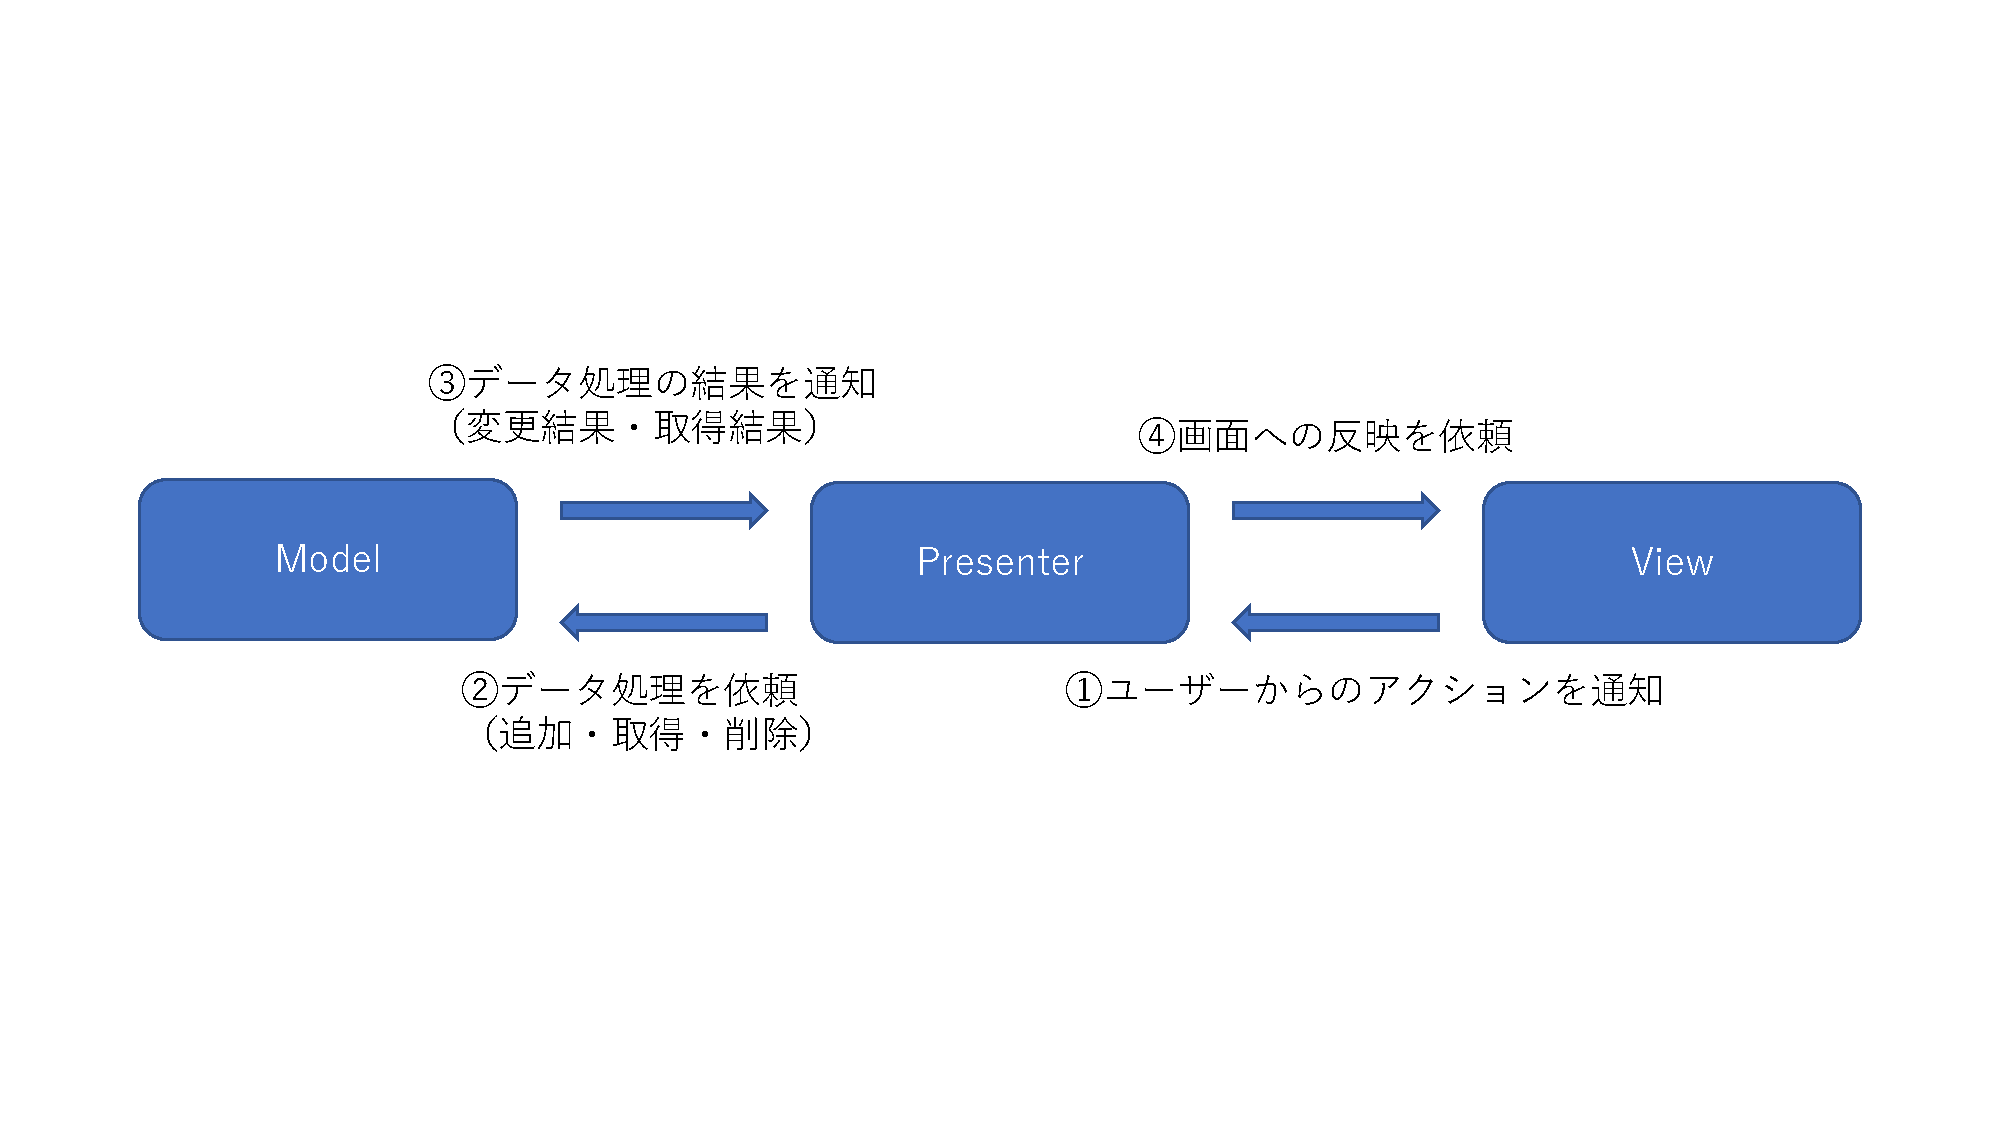
\includegraphics[scale=0.35]{images/mvp_architecture.pdf}
    \caption{MVPアーキテクチャの概念図}
\end{figure}


\subsection{DAOパターンの導入}
今回は,データベースへのアクセスを一括して担うデザインパターンであるDAOを導入した.
全てのデータ処理において,必ずDAOを通すことによって,他のクラスにデータベースアクセスメソッドが分散することを防ぐことができる.
さらに,Modelとしての機能を担っていると考えられるため,PresenterのみがDAOインスタンスを握るように設計した.
ただし,テキストファイルの使用が課題の条件として提示されていたため,通常アプリケーション開発では行われないテキストファイル-データベース間の処理機構も必要となった.
これに対処するために,今回は通常のDAOに加え,テキストファイル-データベース間の処理を担当するTextDAOを設計した.
これら二種類のDAOの分類は,以下の考えに基づいて明確に規定される.
\begin{description}
\item[DAO] 通常のデータベースアクセス処理を担い,今回はデータの追加・取得・削除を行うメソッドを取りまとめている.
\item[TextDAO] データベースをテキストファイルの一次キャッシュとみなし,テキストファイル-データベース間の読み書きを担当する.具体的には,GUI起動時にテキストファイルからデータベースへのデータを読み込み,GUI終了時にデータベースからテキストファイルへのデータ書き込みを行う.結果として,テキストファイルとデータベースの一貫性を保つこととなる.
\end{description}
以下にDAOパターンの概念図を示す. \\
\begin{figure}[!hbt]
    \centering
    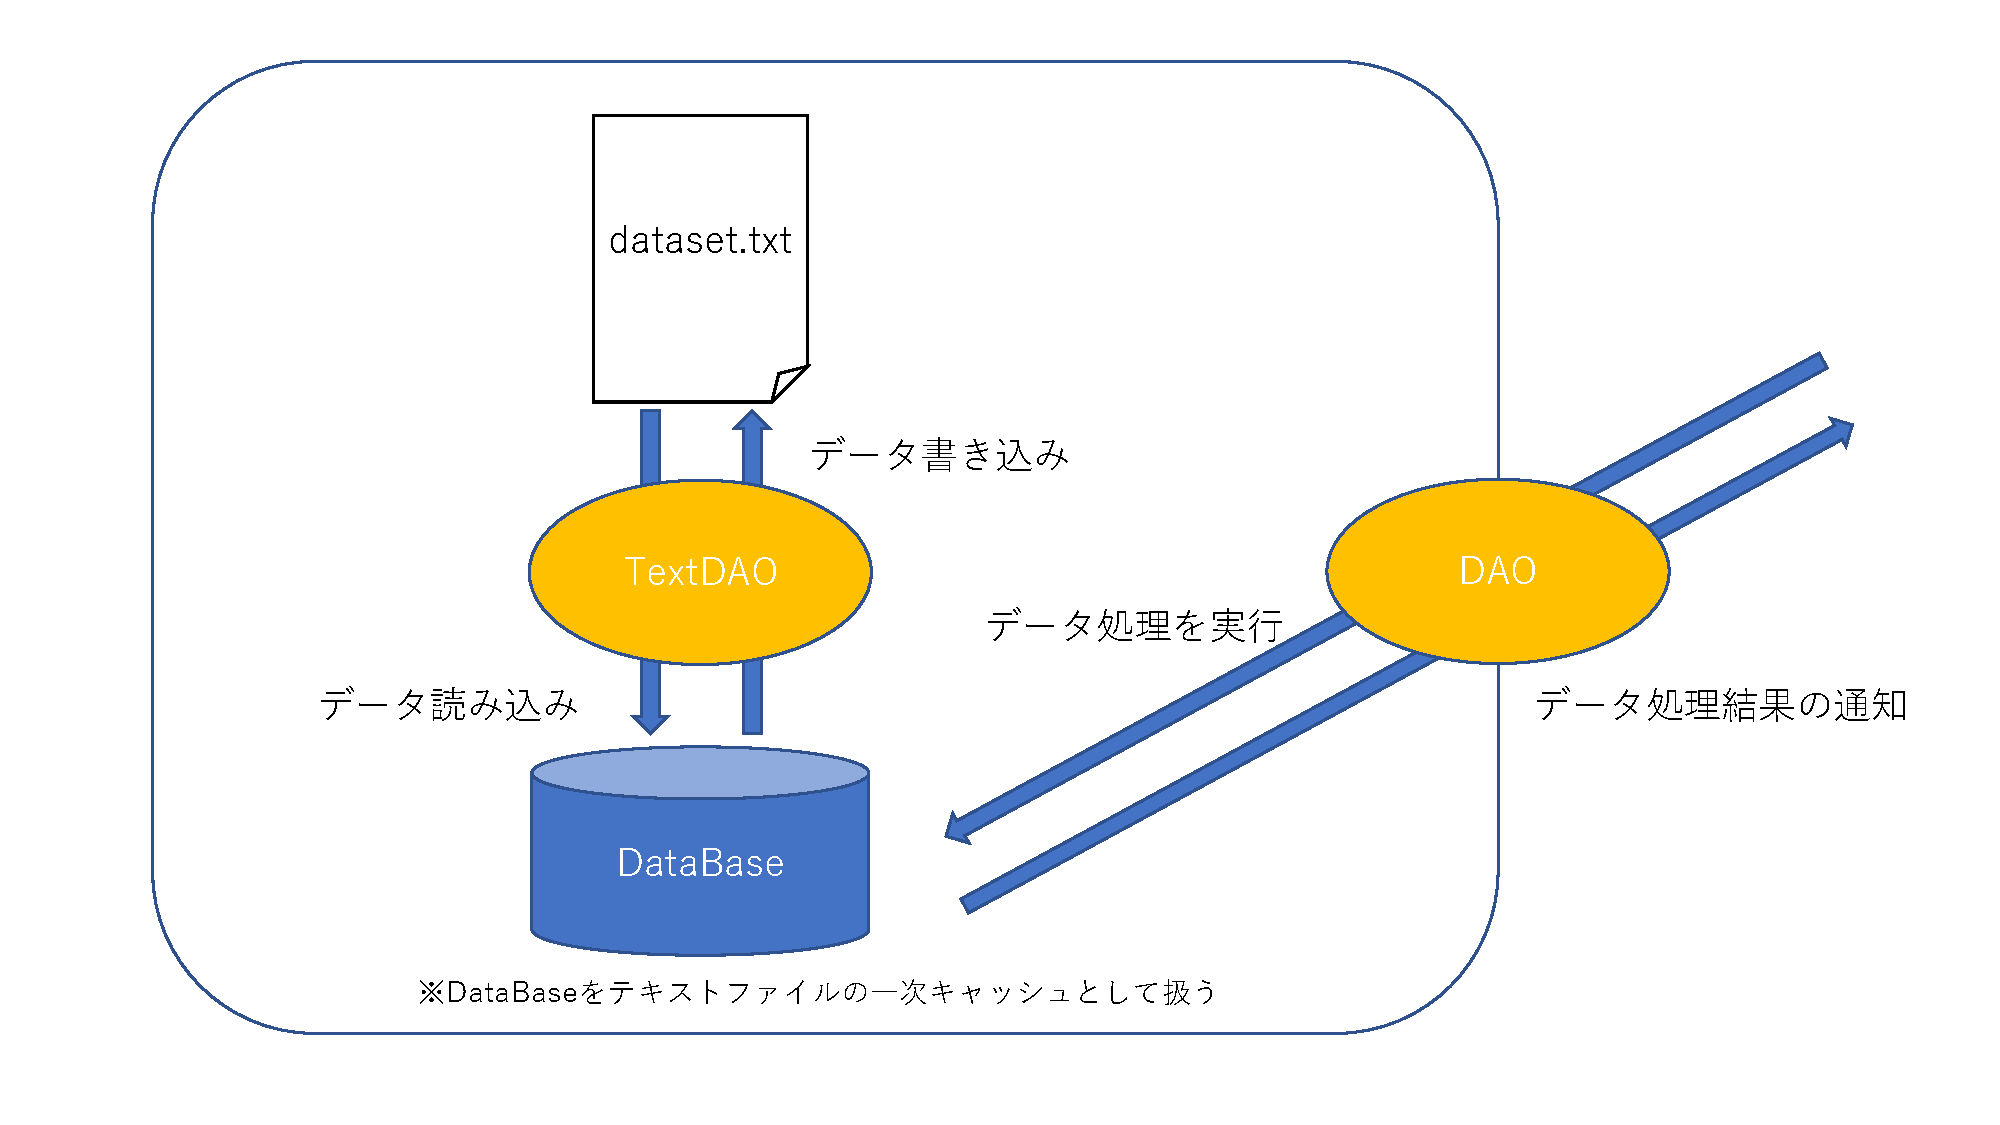
\includegraphics[scale=0.35]{images/dao_pattern.pdf}
    \caption{DAOパターンの概念図}
\end{figure}

\noindent
今回,PresenterはTextDAOに対して以下のメソッドを要求する.
\begin{description}
    \item[readTextFileメソッド] テキストファイルからデータベースへのデータ読み込み
    \item[writeTextFileメソッド] データベースからテキストファイルへのデータ書き込み
\end{description}
PresenterはDAOに対して以下のメソッドを要求する.
\begin{description}
    \item[addDataメソッド] データベースにデータを追加する
    \item[fetchDataListメソッド] データベースからデータを取得する
    \item[deleteDataメソッド] データベースからデータを削除する
\end{description}

\subsection{抽象化による疎結合な関係の構築}
まず,MVPアーキテクチャにおける各要素の間の依存関係について述べる.
上述した通り,ModelクラスはPresenterやViewに全く依存していない.
一方で,PresenterがModelインスタンスを握っていることから,PresenterはModelに依存する関係にある.
加えて,MVPアーキテクチャ含め,一般的なMVC系統のアーキテクチャにおいては,ViewがController部のインスタンスを握ることから,今回はViewがPresenterインスタンスを握ることとなる. \\
ここで,MVPアーキテクチャの特徴として,Presenterはユーザー入力をModelに通知するだけで無く, 直接Viewへの反映命令を行う点があげられることに注目する.
後者の機能の実現には,何らかの形でPsesenterからViewメソッドを呼び出す必要性が生じる.
したがって,Presenter内において,Viewメソッドを持ちうるインスタンスの生成が不可避的となる. \\
しかし,ViewとPresenterが直接互いのインスタンスを握り合うことは望ましく無い.
何故ならば,これらの要素が互いのインスタンスをにぎり合うことにより,強結合と呼ばれる相互的な依存関係が生まれ,アーキテクチャを採用することによる機能分割の意味が薄れるためである.
実際,互いに直接インスタンスを握り合うのであれば,アーキテクチャという観点からはクラスを統一した場合と意義的にはほぼ等しい. \\
この問題を解決するための手法が,インターフェースを利用した抽象化による疎結合な関係の構築である.
実装としては,PresenterからViewを管理するメソッドを集めたViewInterfaceを定義し,Presenter側ではViewInterface型インスタンスを持つようにする.
\begin{lstlisting}[caption=ViewInterfaceの定義, label=mid]
    interface ViewInterface {
        \\データベース初期化完了メソッド
        void successStart();
        \\テキストファイル記録完了メソッド
        void successFinish();
        \\データ追加完了メソッド
        void successAddData();
        \\検索結果反映メソッド
        void showSearchResult(List<TextModel> resultList);
        \\データ削除メソッド
        void successDeleteData();
        \\一覧表示メソッド
        void showResultList(List<TextModel> resultList);
        \\例外処理表示メソッド
        void showError(String errorText);
        \\データ無し表示メソッド
        void showNoData();
    }
\end{lstlisting}
\begin{lstlisting}[caption=PresenterにおけるViewInterface型インスタンスの生成, label=mid]
    class Presenter {
        ...
        private ViewInterface view;

        public Presenter(ViewInterface view) {
            this.view = view;
        }
        ...
    }
\end{lstlisting}
View側の実装クラスでは,インターフェースを実装し,オーバーライドされたメソッドの具体的な処理を記述する.
\begin{lstlisting}[caption=GUIにおけるPresenterインスタンス生成, label=mid]
    class GUI implement ViewInterface {
    ...
    Presenter presenter;
    init() {
        presenter = new Presenter(this);
    }
    ...
}
\end{lstlisting}
また,Viewは生成後にPresenterコンストラクタに自身を渡すことで,Presenterインスタンスを生成する.
反対にViewの終了時には,Presenterインスタンスを離すように設計する. \\

以上により,ViewがPresenterインスタンスを握ることで依存しながらも,Presenter側は直接明示的にViewインスタンスを握らずともViewメソッドを呼び出せる状態が完成する.
すなわち,ViewがPresenterを持つという一方的な依存関係としての疎結合な関係の構築が達成される. \\
結果的に,一般的にアーキテクチャを採用する際に好ましいとされる緩やかな関係性を持たせることができるのである. \\
以下に,View-Presenter間における疎結合な関係を示す.
\begin{figure}[!hbt]
    \centering
    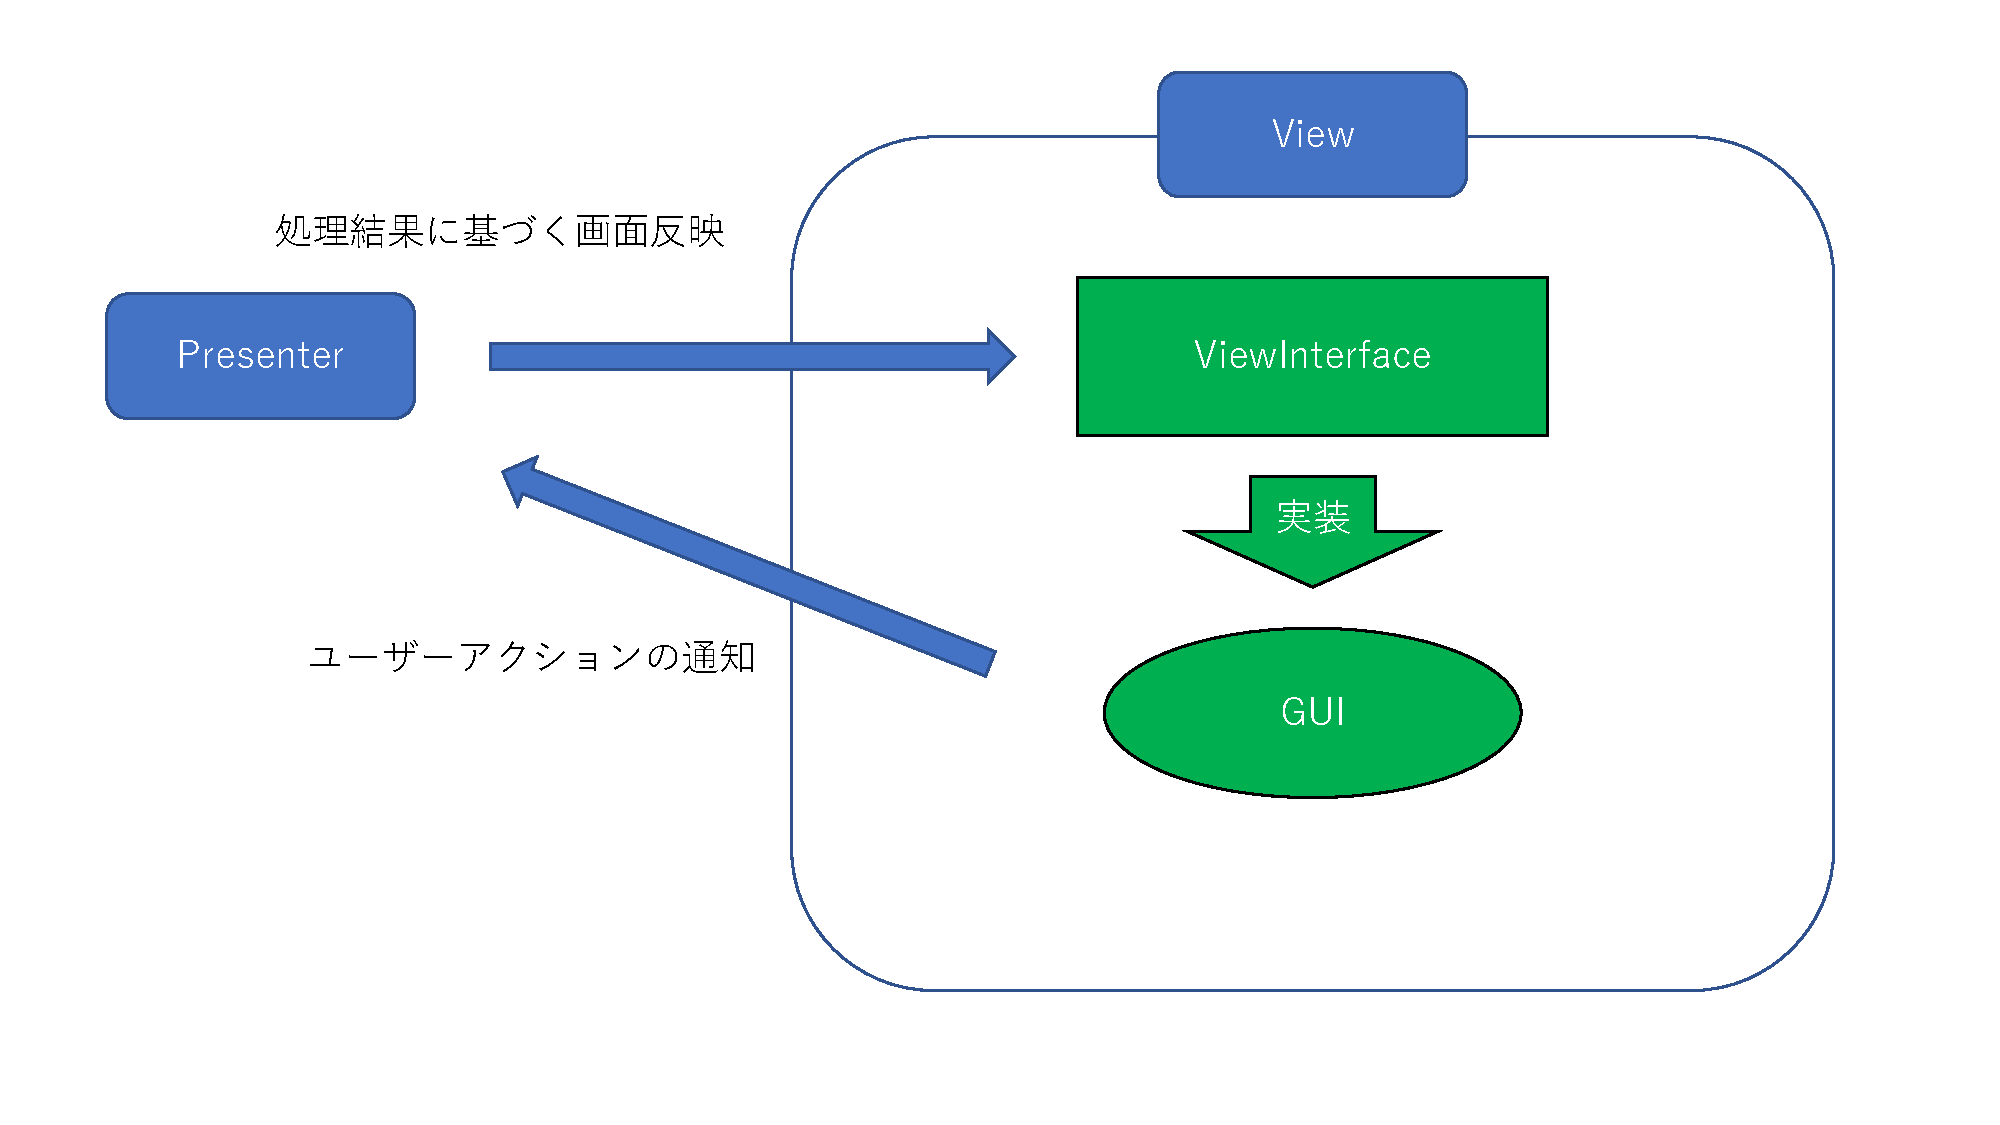
\includegraphics[scale=0.35]{images/view.pdf}
    \caption{View内部とPresenterの依存関係の概念図}
\end{figure}

\newpage

\subsection{システムの全体像}
上述した3種類の技術を用いて,今回の課題のシステムを実現した.
その全体像を以下に示す.
\begin{figure}[!hbt]
    \centering
    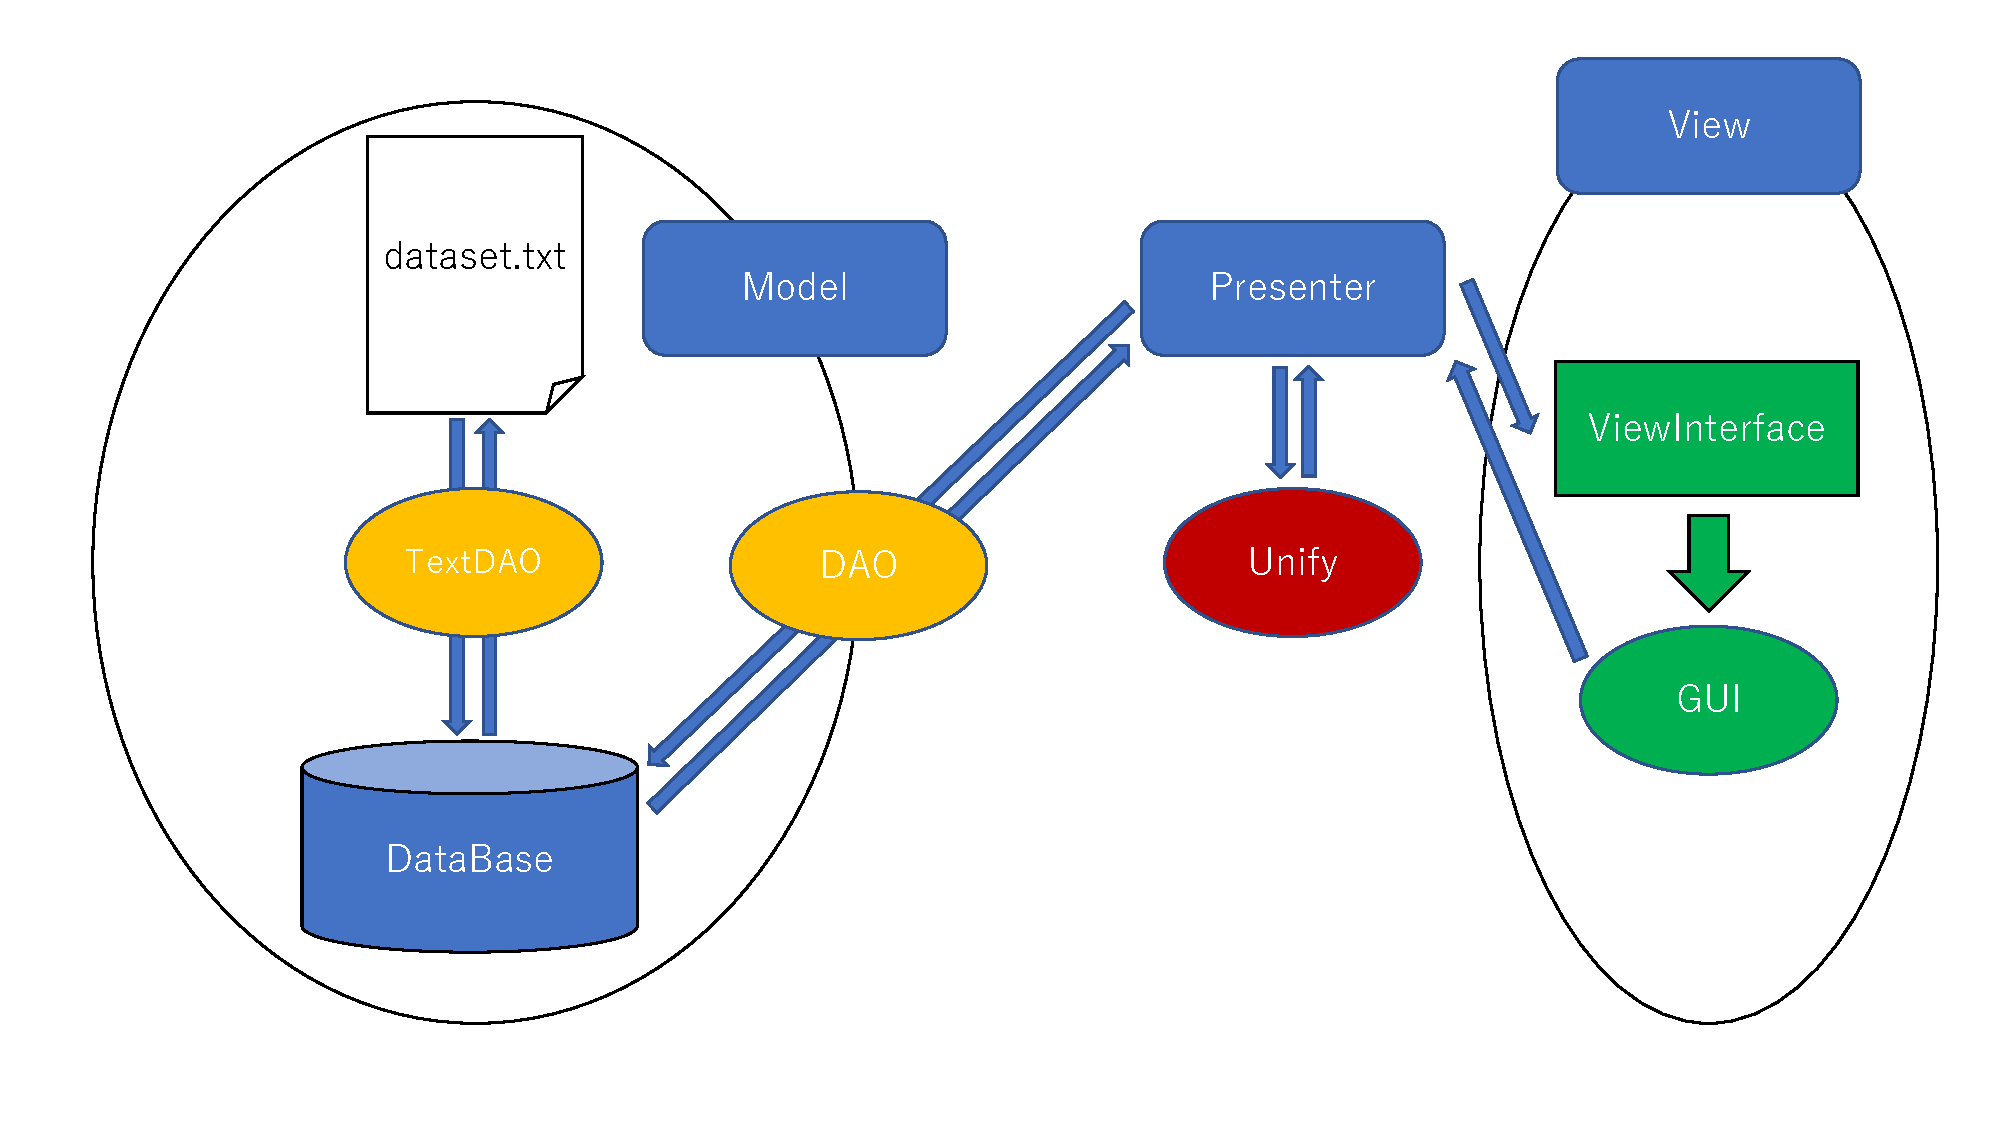
\includegraphics[scale=0.35]{images/architecture_all.pdf}
    \caption{システム全体の概念図}
\end{figure}

\subsection{データ追加・削除機能の実装}
Viewがユーザー入力を受け取り,Presenterに通知する.
PresenterはDAOに問い合わせ,結果により呼び出すViewメソッドを切り替えてViewに反映指示を出す.

\subsection{データ検索・一覧表示機能の実装}
Viewがユーザー入力を受け取り,Presenterに通知する.
PresenterはDAOに問い合わせ,結果として受け取ったデータリストとユーザー入力から得られた文字列をUnify内部のメソッドに渡すことで検索を行う.
Unifyによる検索結果から,呼び出すViewメソッドを切り替えてViewに反映指示を出す.

\subsection{テキストファイル-データベース間の読み込み/書き込み機能の実装}
Viewがユーザー入力を受け取り,Presenterに通知する.
PresenterはTextDAOに問い合わせ,実行結果により呼び出すViewメソッドを切り替えてViewに反映指示を出す.


\subsection{考察}
ここでは,全体的な考察について述べることとする. \\
まず,アプリケーション/システムとして重要なのは機能を明確に区分することであると考えた.
次に,チーム開発を行うに当たって,保守性や可読性を高めることに重点を置くべきだと考えた.
これら二つの考えを基として,MVPアーキテクチャやDAOパターンの導入が適切であると判断した.
その反面,概念的な要素が多く,チームメンバーに対しての説明を要した.
しかし,GitHub上でソースコード管理を行っているので,コンフリクションを防止するためにもアーキテクチャやデザインパターンにより役割分担を行うことは非常に有効な手段であると考えられる. \\

さて,機能の切り分けと分担を考える上では非常に良い課題であると感じた反面,今回の課題について,非常に違和感を感じた点がある.
それは,課題2-3において,テキストファイルへのデータ読み込みと書き出しによりデータの保管を行う指示があることだ.
私は,今までAndroidアプリケーションの開発に携わってきたが,まずデータ保管のためにテキストファイルを用いるのは一般的では無いとの認識を持っている.
通常,サーバーに管理を任せるか,OS標準搭載のデータベースを用いる.
今回であれば,課題2-1でデータベースの作成を要求されているので,データベースを利用するのみで十分であると考えられる.
また,データベースの永続性の観点から,わざわざテキストファイルへの保存を行うのは冗長であると感じられる.
課題の指示内容の解釈に苦しんだので,グループメンバーがTAに質問して提案された内容を重んじ,データベースをテキストファイルの一次キャッシュのような形にすることを決定した.
上述した通り,データベースの利用法としては非常にナンセンスだと感じられる. \\
次に,Unifyとデータベースの検索機能が競合する点である.
Unifyは読み込んだデータを元に指定された文字列とのマッチングを行うことで検索を行う.
一方で,データベースに動詞ごとのテーブルを作り,主格と目的格を属性として持たせ,SELECT文を実行することで同様の機能を実装できる.
すなわち,検索機能に関して二つの実装方式が可能であり,問題文からはUnifyを用いる実装,一般的にはデータベースを用いる実装があげられる.
前者を採用した場合は,データベースはただ一つのみのテーブルを持ち,そのまま文章を格納するだけの機能となり,十分にデータベースを活用できているとは言えない.
後者を採用した場合は,そもそもUnifyを利用する必要性が無くなり,課題の趣旨に反する可能性がある.
結果的に,今回の課題テーマにあるパターンマッチングを活かすために前者を採用したが,現実的な開発においては後者が最適であると個人的に強く感じる. \\
これらのような課題指示の曖昧性と現実的なシステムからの乖離は学生を非常に混乱させ,メンバー間の意思疎通をいたずらに困難とすると考えられる.
もちろん,実装課題であるので,受け手側の受け取り方による多少の揺らぎは許容されるべきであるが,学生の知識や経験にそぐわない実装を手段として選ばざるを得ないような表現にはいささか疑問が残る.
課題内容の吟味と説明の徹底を行うことを強く推奨すると共に,このように学生が解釈に手間取る可能性を十分に考慮して,課題内容を早期に公開すべきであると考える.


\section{発展課題2-3}
\begin{screen}
  上記システムの GUI を作成せよ. \\
・データの追加,検索,削除を GUI で操作できるようにすること. \\
・登録されたデータが次回起動時に消えないよう, 登録されたデータをファイルへ 書き込んだり読み込んだりできるようにすること.
\end{screen}
私は登録されたデータが次回起動時に消えないよう,登録されたデータをファイルへ書き込むことが出来るようにするためのメソッドの作成と,GUIからのDBアクセスのために作成したDao.javaの実装を行った.

\subsection{手法}
必須課題2-1で,テキストファイルからデータセットを読み込むときに利用したTextCon.javatとTextDAO.javaを利用して新しい機能を追加した.追加したものは以下のようになっている.

\begin{enumerate}
\item GUIからの命令で書き換えが行われたDBから,データを取得する.
\item DBから取得したデータを,テキストファイルに書き込む.
\end{enumerate}
これらの実装を私が担当した.

\subsection{実装}
書き換え終了後にDBからその内容を取得するメソッドgetDBData,取得したデータをテキストファイルに書き戻すメソッドwriteTextFileの作成を行った.それぞれのメソッドは,getDBDataメソッドがTextDAO.javaに,writeTextFileメソッドがTextCon.javaに含まれている.\\

取得したデータをテキストファイルに書き戻すメソッドwriteTextFileの実装をソースコード\ref{writeTextFile}に示す.
\begin{lstlisting}[caption=writeTextFileメソッド,label=writeTextFile]
public void writeTextFile() throws FileNotFoundException{
	try {    // ファイル読み込みの操作
		・・・
		// データの取得【DB】
		TextData = TextDAO.getDBData();
		TextDAO.conCom();
		// ファイルへの書き込み
		for (int i = 0 ; i < TextData.size() ; i++){
			out.println(TextData.get(i));
		}
		out.close();        // ファイルを閉じる
	} catch (IOException e) {
		e.printStackTrace();
	}
	TextDAO.closeConn();
}
\end{lstlisting}

DBに格納されているデータを取得するメソッドgetDBDataの実装をソースコード\ref{getDBData}に示す.
\begin{lstlisting}[caption=getDBDataメソッド,label=getDBData]
// DBのデータを取得
public static ArrayList<String> getDBData() {
	conn = null;
	ArrayList<String> DBList = new ArrayList<String>();
	PreparedStatement pStmt = null;
	ResultSet rs = null;
	String sql;
	try{
		Class.forName("org.sqlite.JDBC");
		if(conn == null){
			conn = DriverManager.getConnection(connDB);
			conn.setAutoCommit(false);
		}
		sql = "select line from texts";
		pStmt = conn.prepareStatement(sql);
		rs = pStmt.executeQuery();
		while (rs.next()) {
			String text = rs.getString("line");
			DBList.add(text);
		}
		rs.close();
		pStmt.close();
	}catch{
	・・・
	}
	return DBList;
}
\end{lstlisting}

これらに加え,増田君が作成してくれたたDBへのアクセスを行うDao.javaのプログラムに対して実際の動作が正しく行われるように修正をしたり,Presenter.javaのDBアクセス指令の改良やデバッグなども行った.

\subsection{実行例}
GUIの作成は青山君が作成したため,ここでは私が実装したファイルの書き込み部分のみに着目して実行例を確認する.必須課題2-1で作成したDB作成テスト時に使用したTest.javaを用い,テキストファイルを読み込んでDBに格納し,値の更新や削除を行った後変更したDBからテキストファイルへと上書きまでの動作が正しく行われたかを確認する.使用するデータセットは,与えられたdataset\_example.txtとした.

dataset\_example.txtを操作するためのText.javaをソースコード\ref{dataset_example}に示す.
\begin{lstlisting}[caption=Text.javaのmainメソッド,label=dataset_example]
public static void main(String arg[]){
	// DBの作成
	Presenter presenter = new Presenter(new View());
	presenter.start();
	// DBの書き換え
	presenter.addData("Mike is a boy");
	presenter.deleteData(1);
	presenter.addData("Mike loves Hanako");
	presenter.deleteData(5);
	presenter.addData("Mike has a hobby of playing tennis");
	presenter.deleteData(20);
	presenter.addData("Mike is a boy");
	// テキストファイルへの上書き
	presenter.finish();
}
\end{lstlisting}

addDataでデータの追加を行い,deleteDataでデータの削除を行う.これらはそれぞれ引数にStringとintを持つ.またstart()でテキストファイルからDBへの書き込みを,finish()でDBからテキストファイルへの上書きを行う.これらはPresenterを経由してからDAOへと命令が伝えられる.これを実行するが,このとき変更された内容は繰り返し利用され,2回目の実行時には1回目の変更内容が反映された状態で新しくプログラムの更新を行わなければならない.それを踏まえ実装を行った実行結果が以下のようになる.\\

上のTest.javaの内容を3回繰り返して得られた結果を以下に順に示す.この時示すのは,結果が反映されたテキストファイルとする.\\

\begin{lstlisting}[caption=実行前のdataset\_example.txt,label=1]
Hanako is a girl
Hanako is a student
student is a kind of human
human is a kind of mammal
Hanako has a hobby of playing video-games
Hanako has a hobby of playing air-guitar
Hanako studies philosophy
Hanako loves Taro

Taro is a boy
Taro is a student
Taro has a hobby of playing video-games
Taro studies informatics
Taro loves Jiro
Taro has a pet named Jiro

Jiro is a boy
Jiro is a dog
dog is a kind of mammal
Jiro has a hobby of playing frisbee
Jiro loves Hanako
\end{lstlisting}

\begin{lstlisting}[caption=1回実行後のdataset\_example.txt,label=2]
Hanako is a student
student is a kind of human
human is a kind of mammal
Hanako has a hobby of playing air-guitar
Hanako studies philosophy
Hanako loves Taro
Taro is a boy
Taro is a student
Taro has a hobby of playing video-games
Taro studies informatics
Taro loves Jiro
Taro has a pet named Jiro
Jiro is a boy
Jiro is a dog
dog is a kind of mammal
Jiro has a hobby of playing frisbee
Jiro loves Hanako
Mike loves Hanako
Mike has a hobby of playing tennis
Mike is a boy
\end{lstlisting}

\begin{lstlisting}[caption=2回実行後のdataset\_example.txt,label=3]
student is a kind of human
human is a kind of mammal
Hanako has a hobby of playing air-guitar
Hanako loves Taro
Taro is a boy
Taro is a student
Taro has a hobby of playing video-games
Taro studies informatics
Taro loves Jiro
Taro has a pet named Jiro
Jiro is a boy
Jiro is a dog
dog is a kind of mammal
Jiro has a hobby of playing frisbee
Jiro loves Hanako
Mike loves Hanako
Mike has a hobby of playing tennis
Mike is a boy
Mike loves Hanako
Mike has a hobby of playing tennis
Mike is a boy
\end{lstlisting}

\begin{lstlisting}[caption=3回実行後のdataset\_example.txt,label=4]
human is a kind of mammal
Hanako has a hobby of playing air-guitar
Hanako loves Taro
Taro is a student
Taro has a hobby of playing video-games
Taro studies informatics
Taro loves Jiro
Taro has a pet named Jiro
Jiro is a boy
Jiro is a dog
dog is a kind of mammal
Jiro has a hobby of playing frisbee
Jiro loves Hanako
Mike loves Hanako
Mike has a hobby of playing tennis
Mike is a boy
Mike loves Hanako
Mike is a boy
Mike is a boy
Mike loves Hanako
Mike has a hobby of playing tennis
Mike is a boy
\end{lstlisting}

\subsection{考察}
Test.javaでは,4つの文の追加と3つの文の削除を行っている.このことから実行結果を確認すると,実行回数が増えるたびにテキストファイルに入っている文章の数が一つずつ増えていることが確認できる.また追加ではMikeに関する情報を加えているが,実行回数が増えるたびにMikeに関する文章の数が増えていることも確認できる.これらのことから,このプログラムは前回実行時の内容を保持したまま正しく次の実行が行えていることが分かった.\par
DB格納時に空行は飛ばして格納するようにしたことから,DBの内容をテキストファイルに格納する場合も空行は残らずに上書きが行われることも分かった.さらに,データの削除はDB格納時に各文章に与えられるid番号によって行われるが,実行するたびにテキストファイルの一番上にある行が消えていることから,DBに格納が行われるたびに与えられるid番号が正しく与え直され,その時のテキストファイルの一文目が削除されてることが確認できた.\\

発展課題ではあったものの,私が担当した範囲は必須課題2-1で作成したプログラムとDBに対しての操作を行うため,実装方法自体は大きく悩むことなく取り組むことが出来た.また,GUIとの連動に必要なメソッドはPresenter.javaによって操作が行われるため,私自身はGUI本体を操作することなくプログラムを動作させることが出来た.これはプログラム作成時のアーキテクチャを明確にしていたことが影響しているため,プログラムを作成する前にアーキテクチャを明確にすることの大切さを強く理解した課題となった.

\section{DB関連についての全体の考察}
ここまで,各課題に対する考察を行ってきたため,ここからは私が担当したDB全体に対する考察を行う.\\

今回の課題はDBを作成するとの課題であったことから,プログラミング応用の講義で利用したsqliteを使用してDBを作成することを考えた.課題の要件を満たすようなDBの形として,最終的に表\ref{tab:ex1}の格納方法を使用した.この理由としては,実装難度と実装期間と発展課題でデータの追加や削除を行う必要があると考えたため,DBを利用するとこれらの実装が行えると考えたからである.しかしこれでは,動作が終了するとDBで読み込んだ内容を最終的にテキストファイルへと保存することになり,DBはデータを保存するという意味では機能しなくなってしまう.DBは本来テキストファイルよりもデータの保存に適したものであるのにも関わらず,DBをテキストファイルのキャッシュのように使用することになってしまい,これではDBを利用する利点が無くなってしまうと考えられた.\par
さらに,DBはtableやカラムを持つことが出来ることもテキストファイルよりも保存方法に幅がある.しかしこの格納方法ではほとんどテキストファイルと同様の保存方法になっており,これもDBを有効に活用できていないと感じられる原因となった.\\

これらを解決するためにも,単語毎で分割し動詞毎でtableを作成したり,単語毎でフィールドに追加していく方法も考えた(必須課題2-1考察参照).しかしこの方法を利用すると,検索時にMatchingクラスやUnifyクラスを利用せずとも,変数が単語の分割された何個目に含まれているかという情報と各単語の内容で比較を行うことで検索が出来てしまうと考えられる.これでは課題の内容を満たしているとは言えないため,この方法は使用しないことを決めた.\\

MatchingクラスやUnifyクラスの利用の観点から考えると,先に検索を行い,その際の検索文とその答えをDBに格納する方法が課題内容も満たしDBも活用できているため最も良いようにも考えられる.しかしこれでは発展課題のデータの追加や削除がDBで行えないため容易には実装出来なくなってしまう.追加や削除が行われたデータセットを最終的に保存しなければならないことを考えると,この方法も課題内容を満たさないと考えた.\\

このような考えから,今回は表\ref{tab:ex1}のように実装を行ったが,やはりDBを活用できているようにはあまり感じられない結果となった.そのため,時間に余裕があれば他の方法での実装も検討してみたいと考えた.例えば,検索文とその答えの格納をDBに行う場合は,初めにテキストファイルを読み込んだ際にその内容をListなどに格納しておき,検索や追加,削除はそのListを利用して行うようにし,最終的には変更されたListの内容をテキストファイルに上書きする形を取ることで,発展課題の内容も満たすことが出来るのではないかと考えた.\par
また,データの追加や削除と課題にあったが,この「データ」とはデータセットを指すのか,検索文(パターン)を指すのかも明確に指定されていないように感じた.今回私たちの班は「データ」をデータセットと考えたが,パターンと考えて実装を行うことも可能であると考えられた.そのため,検索文(パターン)とその答えを格納するDBの作成は,課題の内容をより満たしたプログラムの作成となるのではないかとも考えた.\\

ここまではDBの定義の仕方について考察したが,ここからは実際に作成したDBの実装について考察する.\\

DBの作成でまず工夫した点は,id番号を引数で指定することなく決定することが出来るようにしたことである.テキストファイルから読み込んで一文ずつDBに格納する際には1で初期化された変数を順にインクリメントすることで実現できる.しかし追加では別のDAOからDBにアクセスするため変数を取得することが難しい.そこでtableのなかで最大のidを取得する関数max(id)を利用するメソッドgetNoを作成することで今使用されている最大のid番号を取得し,それを1増やした値を追加されたデータのid番号とした.\\

また,作成されたDBの扱い方についても工夫を行った.初めに作成したプログラムでは,同じtable名を作成しようとするとエラーが発生するため,一度実行して作成したDBは次の実行の前に自分で削除しなければならなかった.これを解決するため,まず作成したDBを実行終了と同時に消すことを考えた.しかしsqliteではDBそのものを消す命令が存在していなかったため,この方法は実現させることが出来なかった.\par
次に,実行終了時にDBではなくtableを消すことを考えた.これはdrop tableという命令で可能であることが分かったので,これを実装したところ,二回目以降の実行ではtableが消えているためエラーが発生しなくなった.しかしこれでは,1回目の実行時に別のmainで実行して残っていたプログラムが存在しているとエラーが発生することが分かった.また,実行終了時にtableを消してしまうため,実行終了時にDBにはデータが残らなくなってしまう.そのため,この方法よりも良い実装を考えた.\par
その結果考えたものが,実行開始時にtableを消去する方法である.しかしこれはtableが存在しなかった時にエラーが発生してしまう.そのためtableの存在の有無を判定しようと調べたところ,tableが存在していないときにだけtableを新しく作成することが出来ることが分かった.ここから,tableを作成した後にその中身を削除することを考えた.そこでdeleteDataメソッドを作成し,tableの中身を全て削除してからテキストファイルのデータを書き込むことが出来るようになった.よってDBの有無にかかわらず,正しく読み込んだテキストファイルの内容を格納することが出来るプログラムを作成することが出来た.\par
これは求めたい結果が得られるまでにかなり遠回りをしてしまったが,プログラム改良のプロセスを体感できたように感じた.\\

今回作成したDBでは,追加の際に既に入っているデータをもう一度追加すると,同一内容でもはじくことなく新しいデータとして格納してしまう.これではデータセットの内容の重複が認められてしまうことになるため,同一内容の文章ははじくための処理を入れるべきだった.MatchingクラスやUnifyクラスを用いれば内容が一致しているかどうかの判断は可能だと感じた.今回は時間がなくできなかったが,追加処理を行う際は現在入っているデータと追加文が重複しているかを確認し,重複していないときにのみデータへの追加を行うように実装したい.\\

また,Moodleの質問掲示板の返信から,そもそも既存のDBを利用せずに課題を解かなければならなかったことが分かった.そのため,今までの考え方を大きく変え自作DBの実装方法を考えなければならなかったが,今回は時間がなく考えることが出来なかった.自作DBの実装方法はまだどのように行えばよいのか明確に分かっていないため,今後のためにもどのような方法が利用できるのか考えていきたい.


\section{発展課題2-3}
\begin{screen}
上記システム(MatchingクラスまたはUnifyクラスを用いた,パターンで検索可能な簡単なデータベース)のGUIを作成せよ.

データの追加,検索,削除をGUIで操作できるようにすること.

登録されたデータが次回起動時に消えないよう,登録されたデータをファイルへ書き込んだり読み込んだりできるようにすること.
\end{screen}
私の担当箇所は,発展課題2-3のGUI全般のSwingを用いた実装である.

\subsection{手法}
GUIを実装するにあたり,以下のような方針を立てた.
\begin{enumerate}
\item データベースとデータのやりとりをするためのクラスやメソッドを作る.
\item 検索・追加・削除のためのテキストフィールドやボタン,リストを表示する.
\item 表示した各種コンポーネントを動作させる.データベースからデータを受け取ってGUIに反映する.
\end{enumerate}

1.に関して,班員と協力してタスクを分割し,データベースとの直接のやり取りはPresenterクラスに任せた.自分はPresenterからデータを受け取るためのViewクラス等を作成して用いることで,より構造化されたデータのやり取りを可能とした.

2.に関して,GridBagLayoutを用いてコンポーネントの配置を行うことで,ユーザがより直感的に利用できるよう工夫した.また,データベースの一覧を表示することで,データの追加・削除・検索の視覚的な確認を行えるような仕様とした.また,削除を一覧から選択して実行できるように,一覧の表示にはJListクラスを用いた.

3.に関して,VIewクラスを介することで,コンソールを通じてGUIに正しく反映できているかを確認できるような仕様とした.また,ボタンを押したと同時にGUI上のリストを更新するために,DefaultListModelクラスを利用した.

\clearpage

\subsection{実装}

実装にあたり,主に下記のサイトを参考にした. \\

TATSUO IKURA: 『Swingを使ってみよう - Java GUIプログラミング』 https://www.javadrive.jp/tutorial/ (2019/10/29アクセス) \\

GUIに大きく関連するプログラムとして,UnifyGUI.java, Presenter.java, TextModel.java, ViewInterface.javaが挙げられる.各プログラムの説明については以下の通りである.

UnifyGUI.javaには以下のクラスが含まれる.
\begin{itemize}
\item SearchGUI: メソッドmain, actionPerformed, クラスmyListenerを実装したクラス.
\item View: インターフェースViewInterfaceを実装したメソッド,各種ゲッターを実装したクラス.
\end{itemize}

Presenter.javaには以下のクラスが含まれる.
\begin{itemize}
\item Presenter: メソッドstart, finish, addData, searchData, deleteData, fetchDataを実装したクラス.
\end{itemize}

TextModel.javaには以下のクラスが含まれる.
\begin{itemize}
\item TextModel: データベースのIDとテキストを一元的に保持するためのクラス.IDとテキストのゲッターを実装している.
\end{itemize}

ViewInterface.javaには以下のクラスが含まれる.
\begin{itemize}
\item ViewInterface: メソッドsuccessStart, successFinish, successAddData, showSearchResult, successDeleteData, showResultList, showError, showNoDataを持つインターフェース.
\end{itemize}

\subsubsection{データベースとデータのやりとりをするためのクラスやメソッドを作るまで}
他の班員が作ったPresenterクラスを介してデータを受け取るために,まずViewInterfaceインターフェースを実装する必要があった.初めはUnifyGUI自体に実装しようと考えたが,Presenterのインスタンスの引数にVIewInterfaceを実装したクラスを渡す必要があったため,こうするとUnifyGUIのmainメソッドを実行しようとしたとき,staticであるため自身を引数として渡すことができなくなるという問題が発生した.

そこで,ViewInterfaceを実装するためのクラスとしてViewクラスを別に作った.ViewクラスではPresenterとのやり取りのたびにコンソールに結果が出力されるため,デバッグ等で活用しやすいものにできた.

また,Presenterクラス側から,プログラム開始時にstartメソッド,終了時にfinishメソッドを呼び出してほしいという要求があったため,WindowAdapterクラスを拡張したmyListenerにおいて,windowOpenedメソッドとwindowClosingメソッドの実装によりこれらを実現した.これにより,ウィンドウが最初に表示されたときにstartメソッドが呼び出され,ウィンドウを閉じようとしたときにfinishメソッドが自動的に呼び出されるように実装した.
myListenerクラスをソースコード\ref{window}に示す.

\begin{lstlisting}[caption=myListenerクラス, label=window]
    public class myListener extends WindowAdapter {
        public void windowOpened(WindowEvent e) {
            view = new View();
            presenter = new Presenter(view);
            presenter.start();
            presenter.fetchData();
            textList = view.getRl();
            for (TextModel text : textList) {
                lModel.addElement(text);
            }
        }

        public void windowClosing(WindowEvent e) {
            presenter.finish();
        }
    }
\end{lstlisting}

\subsubsection{検索・追加・削除のためのテキストフィールドやボタン,リストを表示するまで}
検索や追加には入力が必要なため,JTextFieldを用いて入力を可能とし,JButtonクラスで対応するボタンの表示を行った.また,検索結果の表示と,データベースの要素の表示にはJListクラスを用いた.

これらのコンポーネントの表示には,ユーザが直感的に扱いやすくするためのレイアウトを考える必要があった.そこで今回の形式に最も適していそうなGridBagLayoutクラスを用いることとした.また,細かな配置を行うためにGridBagConstraintsクラスを用いた.このクラスのフィールドであるgridxやgridyでセルを設定したり,anchorでセル内の配置を調整することで,ユーザにわかりやすいレイアウトの構築ができた.
これをソースコード\ref{layout}に示す.

\begin{lstlisting}[caption=UnifyGUIコンストラクタの一部, label=layout]
        gbc.gridx = 0;
        gbc.gridy = 0;
        layout.setConstraints(text, gbc);

        gbc.gridy = 1;
        gbc.anchor = GridBagConstraints.NORTHEAST;
        layout.setConstraints(btnPanel, gbc);

        gbc.gridy = 2;
        gbc.anchor = GridBagConstraints.CENTER;
        layout.setConstraints(searchSp, gbc);
        ...
        gbc.gridx = 1;
        gbc.gridy = 0;
        gbc.gridheight = 3;
        layout.setConstraints(listSp, gbc);

        gbc.gridy = 3;
        gbc.gridheight = 1;
        gbc.anchor = GridBagConstraints.NORTHEAST;
        layout.setConstraints(delButton, gbc);
\end{lstlisting}

\subsubsection{表示した各種コンポーネントを動作させたり,データベースからデータを受け取ってGUIに反映したりするまで}
ボタンが押下されたときに入力データを引数としてPresenterからメソッドを呼び出すことを,ActionListenerインターフェースのactionPerformedメソッドの実装により実現した.このとき,どのボタンが押されたかを判別するために,getActionCommandメソッドを用いた.

削除においては,リストから選択して行えるように,getSelectedIndexメソッドを利用して,どの項目が選択されているかの取得を行い,Presenterへの引数として渡した.

これらを行うactionPerformedメソッドをソースコード\ref{act}に示す.

\begin{lstlisting}[caption=actionPerformedメソッド, label=act]
    public void actionPerformed(ActionEvent e) {
        String cmd = e.getActionCommand();
        String arg = text.getText();

        if (cmd.equals("検索")) {
            presenter.searchData(arg);
            sModel.clear();
            searchList = view.getSr();
            for (String text : searchList) {
                sModel.addElement(text);
            }

        } else if (cmd.equals("追加")) {
            presenter.addData(arg);
            lModel.clear();
            presenter.fetchData();
            textList = view.getRl();
            for (TextModel text : textList) {
                lModel.addElement(text);
            }

        } else if (cmd.equals("削除")) {
            if (!listPanel.isSelectionEmpty()) {
                int index = listPanel.getSelectedIndex();
                TextModel val = (TextModel) listPanel.getSelectedValue();
                presenter.deleteData(val.getUUID());
                lModel.remove(index);
            } else {
                System.out.println("削除失敗(未選択のため)");
            }
        }
    }
\end{lstlisting}

このソースコードに示されたように,リストへの表示はDefaultListModelクラスのaddメソッドを用いて行った.
また,ソースコード\ref{window}のstartメソッド内でも同様の処理が行われており,リストの初期状態,すなわちデータベースの初期状態がウィンドウ表示時に反映されている.

また,このソースコードから分かるように,データの要求はPresenterに対して行っている一方で,データの受け取りはViewを介して行っている.これはデータベースの保守性を高めるための,Presenterクラス担当者の意向によるものである. \\

もしリストの中身が多くなり,画面内に全ての要素が一度で表示しきれないときにスクロールバーを表示するために,JScrollPaneクラスを用いた.JListインスタンスをこのコンポーネント内に入れることで,期待通りの実装ができた.この際,コンポーネントを思った通りのサイズにするために,setPreferredSizeメソッドで調整した.
これをソースコード\ref{scroll}に示す.

\begin{lstlisting}[caption=UnifyGUIコンストラクタの一部, label=scroll]
        sModel = new DefaultListModel();
        searchPanel = new JList(sModel);
        JScrollPane searchSp = new JScrollPane();
        searchSp.getViewport().setView(searchPanel);
        searchSp.setPreferredSize(new Dimension(200, 300));
        ...
        mainPanel.add(searchSp);
\end{lstlisting}


\clearpage
\subsection{実行例}
UnifyGUIを実行したところ,下図のような画面が得られる.

\begin{figure}[!hbt]
  	\begin{center}
  		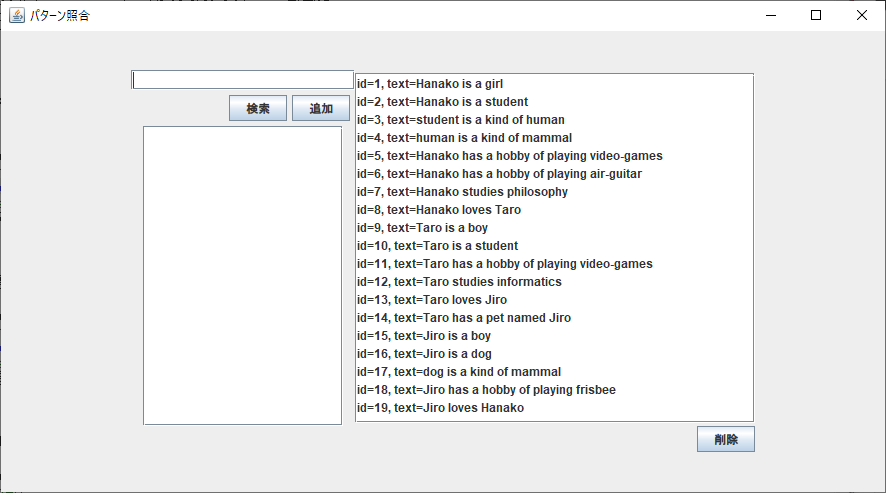
\includegraphics[scale=0.60]{images/scs2-3-1.png}
	\end{center}
  	\caption{初期状態}
\end{figure}
\clearpage

Matchingに関する質問文「?x has a hobby of playing video-games」を入力し,検索ボタンを押したところ,下図のような画面が得られる.

\begin{figure}[!hbt]
  	\begin{center}
  		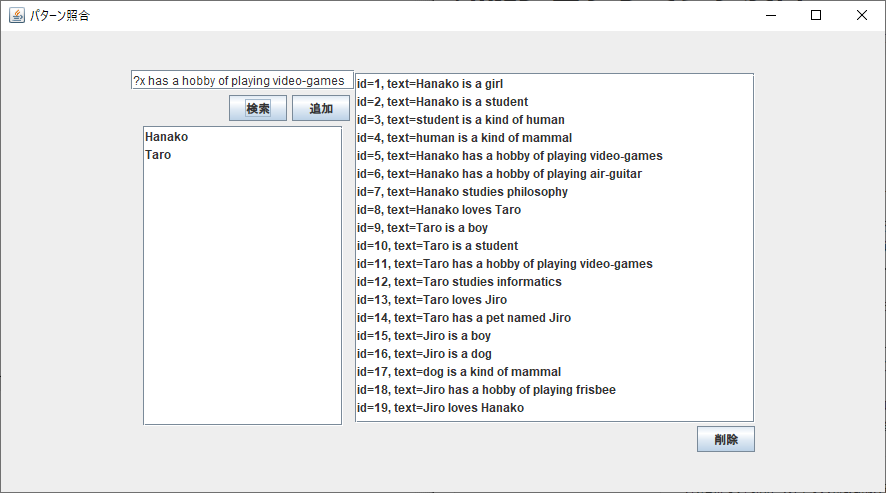
\includegraphics[scale=0.60]{images/scs2-3-2.png}
	\end{center}
  	\caption{Matchingの検索}
\end{figure}
\clearpage

Unifyに関する質問文「?x is a boy,?x loves ?y」を入力し,検索ボタンを押したところ,下図のような画面が得られる.

\begin{figure}[!hbt]
  	\begin{center}
  		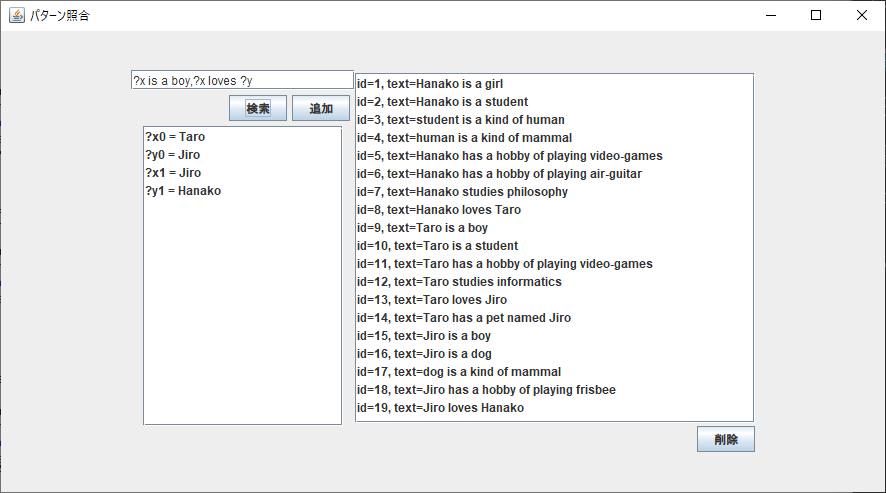
\includegraphics[scale=0.60]{images/scs2-3-6.png}
	\end{center}
  	\caption{Unifyの検索}
\end{figure}
\clearpage

データ「Shuhei is a boy」を入力し,追加ボタンを押したところ,下図のような画面が得られる.

\begin{figure}[!hbt]
  	\begin{center}
  		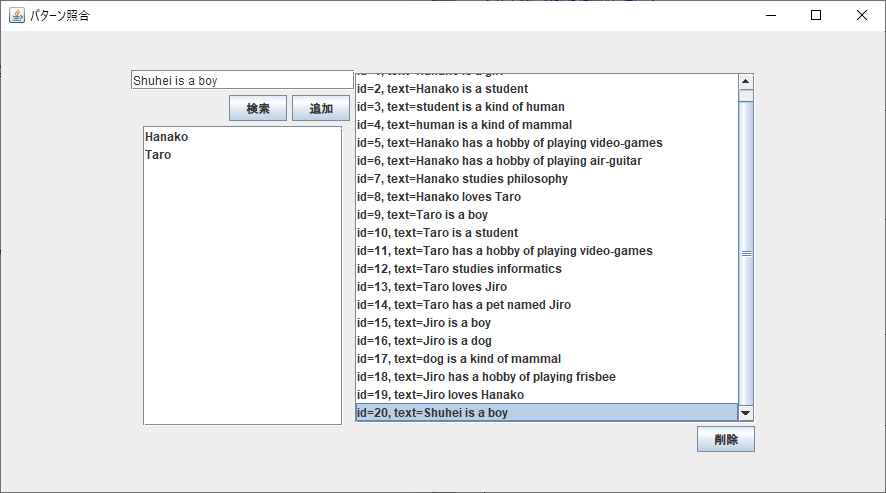
\includegraphics[scale=0.60]{images/scs2-3-3.png}
	\end{center}
  	\caption{データの追加}
\end{figure}
\clearpage

右のリストから「id=19,text=Jiro loves Hanako」を選択し,削除ボタンを押したところ,下図のような画面が得られる.

\begin{figure}[!hbt]
  	\begin{center}
  		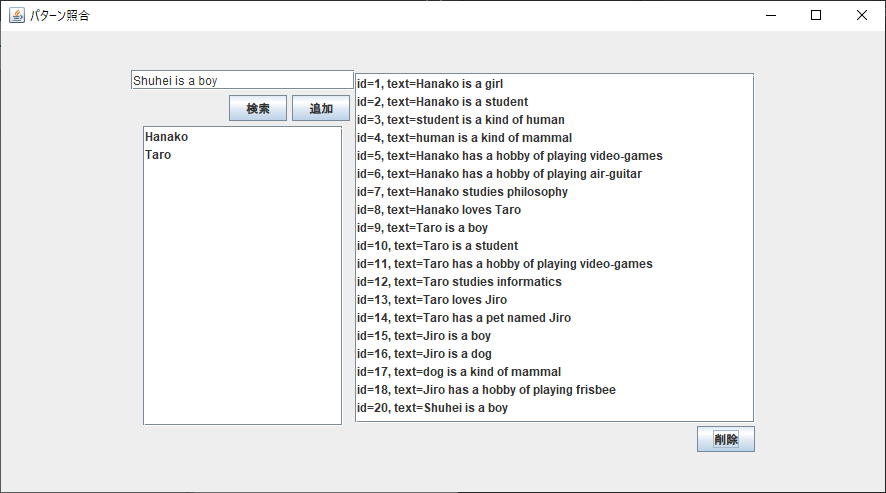
\includegraphics[scale=0.60]{images/scs2-3-4.png}
	\end{center}
  	\caption{データの削除}
\end{figure}
\clearpage

右上の「×」ボタンからプログラムを終了し,再度UnifyGUIを実行して起動したところ,下図のような画面が得られ,前回の追加・削除したデータが保持されていることが分かる.

\begin{figure}[!hbt]
  	\begin{center}
  		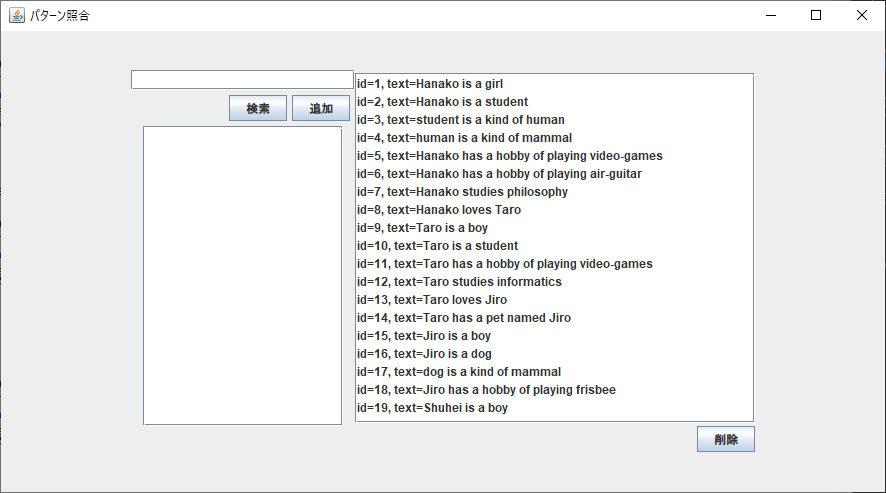
\includegraphics[scale=0.60]{images/scs2-3-5.png}
	\end{center}
  	\caption{プログラムの再起動}
\end{figure}
\clearpage

\subsection{考察}
ViewInterfaceを実装するためのクラスとしてViewクラスをUnifyGUIクラスとは別に作ったが,これによりPresenterからの値をGUI実行時に使えるようになっただけでなく,UnifyGUIクラスを介さずともUnifyクラス等の単体テスト時にもPresenterクラスを利用できるようになったため,結果として独立したクラスでViewInterfaceを実装してよかったと考えられる.

また,Presenter担当者からの要求としてstart,finishメソッドの実行をプログラム開始・終了時に求められたが,finishメソッドの呼び出しにおいて,windowClosingメソッドの他に,windowClosedメソッドの利用が候補として挙げられた.しかし,windowClosedメソッドではfinishメソッドの呼び出しが行われなかったため,windowClosingメソッドを用いることとなった.windowClosingメソッドはウィンドウをクローズしようとしたときに呼び出される機能である一方で,windowClosedメソッドはウィンドウがクローズされたときに呼び出される機能であるが,いずれにおいてもウィンドウはクローズされるのに,なぜwindowClosedメソッドではfinishメソッドが呼び出されないのかは,ウィンドウがクローズした後finishメソッドを呼び出す前にUnifyGUIプログラムが終了してしまうためだと考えられる.要するに,「×」ボタンが押された時にプログラムを終了させるために設定したsetDefaultCloseOperation(JFrame.EXIT\_ON\_CLOSE)の方が,windowClosedメソッドよりも実行優先度が上であるためだと考えられる.
また,コンソールから「Ctrl+C」でプログラムを強制終了した場合も,finishメソッドは呼び出されなかったため,強制終了はwindowCloseingメソッドよりも優先度が高いことが分かった.

GUIの表示において,レイアウトの設定が大変であった.setPrefferdSizeやsetMaximumSize等のメソッドを駆使しても,コンポーネントを意図した通りの配置や大きさにすることが難しかった.そこで,GridBagLayoutクラスを用いたところ,これらの問題を一同に解消することができた.GridBagLayoutは表形式でありながらも相対的な位置を高い自由度で配置することができるため,今後も自由な表形式のGUIを作りたいときに重宝すべきものであると考えられた.

JListにスクロールバーを追加するためにJScrollPaneクラスを用いたが,これによりペインにも様々な種類があることを認識できた.JScrollPaneクラスを用いて実際に実装してみることで,ペインはパネルを多機能化したものというような認識を得ることができた.

今回のプログラムでは,データベース担当,GUI担当,これらの仲介担当といったようにグループ内で分担を行ったが,この並行作業は大変なものであった.自分の知らないところでプログラムの構造が想定していたものから変わっていることがあり,グループ内で作業進捗の共有をより密に行う必要があったと感じたと同時に,プログラムが大規模になってくると,どうしても自分の干渉できない部分が出てくることは仕方のないことと割り切り,自分の想定していたものとは異なっていてもこちらが相手に合わせてあげるといったことも重要だと考えられる.

しかし,今回の他の班員が作ったデータベースの構成についてはもう少し言及すべきだったと反省している.今回のデータベースはキャッシュとして扱われており,これは永続的な記憶を目的とするデータベースの本来の用途とは異なっていると考えられる.また,データベースの構造自体も,各行にIDを割り振って1つのレコードとして取り扱うという,文が構造化されて分解されたものだとは到底言い難いものとなってしまったと考えられる.

\begin{thebibliography}{99}
\bibitem{notty} Javaによる知能プログラミング入門 --著:新谷 虎松 \\
\bibitem{notty} java CSV出力 --著:TECH Pin \\
\url{https://tech.pjin.jp/blog/2017/10/17/【java】csv出力のサンプルコード}
\bibitem{notty} Webアプリケーション開発者から見た、MVCとMVP、そしてMVVMの違い (Qiita) --著:shinkuFencer \\
\url{https://qiita.com/shinkuFencer/items/f2651073fb71416b6cd7} (2019年10月25日アクセス). \\
\bibitem{notty} 開発者が知っておくべき、6つのUIアーキテクチャ・パターン ―― 「matarillo.com」より ―― (.NET開発者中心 厳選ブログ記事) --著:猪股 健太郎 \\
\url{https://www.atmarkit.co.jp/fdotnet/chushin/greatblogentry_10/greatblogentry_10_01.html} (2019年10月25日アクセス). \\
\bibitem{notty} お前らがModelと呼ぶアレをなんと呼ぶべきか。近辺の用語(EntityとかVOとかDTOとか)について整理しつつ考える (Qiita) --著:takasek \\
\url{https://qiita.com/takasek/items/70ab5a61756ee620aee6} (2019年10月25日アクセス). \\
\bibitem{notty} Java SQLiteにJDBC接続してinsert/update/deleteするサンプル (ITSakura) \\
\url{https://itsakura.com/java-sqlite-insert} (2019年10月25日アクセス). \\
\bibitem{hanako} プログラミング応用で作成したDAO等のプログラム
\bibitem{notty} RUGBY WORLD CUP, \url{https://www.rugbyworldcup.com/} (2019年10月29日アクセス).
\bibitem{notty} DBOnline SQLite入門, \url{https://www.dbonline.jp/sqlite/} (2019年10月29日アクセス).
\bibitem{notty} memocarilog, \url{https://memocarilog.info/php-mysql/5355} (2019年10月29日アクセス).
\bibitem{notty} プログラミングマガジン 【デザインパターン】DAO/DTOパターン, \url{www.code-magagine.com/?p=1311} (2019年10月29日アクセス).
\bibitem{notty} CMOクラウドアカデミー データベースの用語を理解しよう 「テーブル」「レコード」「カラム」「フィールド」とは?, \url{https://academy.gmocloud.com/know/20160425/2259} (2019年10月29日アクセス).
\end{thebibliography}

\end{document}